\documentclass[a4paper,10pt]{book}

\usepackage[utf8]{inputenc}
\usepackage[T1]{fontenc}
\usepackage{lmodern}
\usepackage[top=3cm, bottom=3cm, left=4cm, right=2cm]{geometry}
\usepackage{amsmath}
\usepackage{amsfonts}
\usepackage{amsthm}
\usepackage{amssymb}
\usepackage{mathrsfs}
\usepackage{graphicx}
\usepackage{wrapfig}
\usepackage{stmaryrd}

\usepackage{url}
\let\urlorig\url
\renewcommand{\url}[1]{\begin{otherlanguage}{english}\urlorig{#1}\end{otherlanguage}}

\usepackage[english,francais]{babel}
\usepackage{tikz}
\usepackage[pdftex, pdfauthor={Pierre Gimalac}, pdftitle={Physique I}, pdfsubject={Physique}, pdfkeywords={licence, mathématiques, physique, mécanique}, colorlinks=true, linkcolor=black, urlcolor=black]{hyperref}
\usepackage{changepage}
\usepackage{pdflscape}
\usepackage[squaren,Gray]{SIunits}

\newcommand{\R}{\mathbb{R}}
\newcommand{\Rpe}{\mathbb{R}_{+}^{*}}
\newcommand{\N}{\mathbb{N}}
\newcommand{\Z}{\mathbb{Z}}
\newcommand{\C}{\mathbb{C}}
\newcommand{\Q}{\mathbb{Q}}

\begin{document}

\begin{titlepage}
\newgeometry{margin=2.7cm}
\thispagestyle{empty}
\begin{center}
\vspace*{7cm}
\Huge \textsc{Physique I}\\
\vspace{1.5cm}
\Large Pierre Gimalac\\
\vspace{0.5cm}
\large \textit{Licence de Mathématiques}
\vfill
\end{center}
\large \textit{Septembre-Décembre 2016}
\hfill 
\large Cours de Cécile de Hosson
\restoregeometry
\end{titlepage}

\renewcommand{\contentsname}{Sommaire}
\thispagestyle{empty}
\tableofcontents \thispagestyle{empty}

\chapter*{Introduction}
\section*{Analyse dimensionnelle}

Chaque membre d'une équation doit avoir la même unité, c'est ce qu'on appelle l'homogénéité.\\

On s’intéresse ici à trois dimensions seulement:
\begin{itemize}
\item T le temps en secondes
\item L la distance en mètres
\item M la masse en kilogrammes\\
\end{itemize}

Il est donc possible de trouver par analyse dimensionnelle les grandeurs physiques dont dépend une autre grandeur physique.\\

\textbf{Exemple:} \emph{la période d'un pendule}\\

On suppose que la période dépend de l'amplitude de départ (angle), la masse du pendule, la longueur du fil et l'intensité du champ de pesanteur.\\

On a donc $T$ $\alpha$ $m^{a}*g^{b}*l^{c}*\theta^{d}$ ($\alpha$ signifie "proportionnel à").\\

$\left \{ \begin{array}{rcl} [T] &=& T \\
\text{[g]} &=& L*T^{-2} \\
\text{[l]} &=& L \\
\text{[m]} &=& M \\
$[$\theta$]$&=& ... \end{array} \right . $\\\\

On cherche a,b,c tel que l’équation ci-dessous soit homogène :

$T=M^{a}*(L*T^{-2})^{b}*L^{c}$ d'où $\left \{ \begin{array}{rcl} a&=&0\\b&=&-\frac{1}{2} \\ c&=&\frac{1}{2} \end{array} \right . $

donc $T$ $\alpha$ $\sqrt{\frac{l}{g}}$.\\

\emph{La véritable formule est} $T=2\pi\sqrt{\frac{l}{g}}$.

\section*{Ordre de grandeur}
L'ordre de grandeur d'un nombre est une estimation à une puissance de 10 de cette valeur.\\

\textbf{Exemples :}
\begin{enumerate}
\item \emph{Le nombre de respiration dans une vie}\\
$n=80*365*24*60*45\approx 100*1000*100*8*6*5 \approx 10^{9}$
\item \emph{Le nombre d'accordeurs de piano a Chicago}
(sachant qu'il y a 5.000.000 d'habitants)\\
\url{https://fr.wikipedia.org/wiki/Estimation_de_Fermi#Exemples_de_probl.C3.A8mes_de_Fermi}
\end{enumerate}

\chapter{Le mouvement, description et cause}
\section*{Définition}
La mécanique est la science du mouvement, il s'agit d'être capable de décrire précisément le mouvement d'un corps dans l'espace, de pouvoir prédire les mouvements et d'en rechercher les causes.\\

\section{Référentiels et référentiels galiléens}
\subsection{Définition}
Le mouvement dépend du référentiel dans lequel il est observé ; un référentiel est un solide indéformable par rapport auquel on repère une position (repère mathématique) ou un mouvement, muni d'une horloge ; ce solide peut être un ensemble d'observateurs immobiles les uns par rapport aux autres.

\subsection{Repérage d'un point M - le vecteur position}

Dans le plan $(O, \vec{i}, \vec{j})$, le vecteur position d'un point M de coordonnées $M(x;y;t)$ est $\overset{\longrightarrow}{OM}$ et \\\\
$\overset{\longrightarrow}{OM} =x\vec{i}+y\vec{j}\\
\overset{\longrightarrow}{OM}=||\overset{\longrightarrow}{OM}||*cos(\theta)*\vec{i}+||\overset{\longrightarrow}{OM}||*sin(\theta)*\vec{j}$\\
\begin{center} \begin{tikzpicture}

\draw[>=latex, ->] (-0.5,0) -- (3,0) ;
\draw[>=latex, ->] (0,-0.5) -- (0,3) ;
\node at (-0.25,-0.25) {0} ;
\node at (2,-0.05) {$\shortmid$} ;
\node at (2,-0.4) {1} ;
\node at (-0.18,2) {1 -} ;
\draw[->, thick] (0,0) -- (1.75,2.3) node[near end, above left] {$\overrightarrow{OM}$} ;
\node at (1.8,2.34) {$\bullet$} ;
\node at (2,2.6) {M} ;
\draw (0.75,0) arc (0:52.5:0.75) ;
\node at (0.8,0.45) {$\theta$} ;
\draw[->, thick] (0,0) -- (2,0) node[midway, below right] {$\vec{i}$} ;
\draw[->, thick] (0,0) -- (0,1.97) node[midway, left] {$\vec{j}$} ;
\end{tikzpicture} \end{center}
La succession des positions de M dans l’espace forme une "trajectoire".\\

\subsection{Vitesse instantanée du point M - le vecteur vitesse}
Le vecteur vitesse $\vec{v}$ du point M représente la vitesse instantanée du point M, il est toujours tangent à la trajectoire de ce point M.\\\\
$\vec{v}=\frac{\Delta\overset{\longrightarrow}{OM}}{\Delta t}=\frac{\Delta x}{\Delta t}\vec{i}+\frac{\Delta y}{\Delta t}\vec{j}$\\
\begin{center}
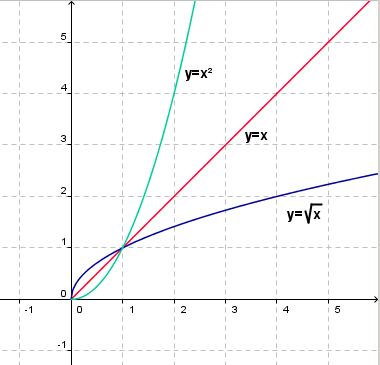
\includegraphics[scale=1.3]{images/002.jpg}
\end{center}

\subsection{Référentiels galiléens (inertiels) et principe d'inertie}
\subsubsection{Définitions}

\paragraph{Référentiel galiléen :} un référentiel galiléen est un référentiel dans lequel le principe d'inertie s'applique.\\

\paragraph{Principe d'inertie :} lorsque la somme des force appliquées a un système est nulle, alors le mouvement de ce système est rectiligne uniforme (système (pseudo) isolé).\\
$\sum \vec{F}_{ext}=\vec{0}$\\

\paragraph{Mouvement rectiligne uniforme :} un système en mouvement rectiligne uniforme possède une vitesse vectoriellement constante (norme et sens), un système au repos est donc en mouvement rectiligne uniforme.\\
Tous les référentiels en mouvement rectiligne uniforme les uns par rapport aux autres sont galiléens (si l'un d'entre eux l'est).\\

\subsubsection{Référentiels communs\\}

\paragraph{Référentiel terrestre :} il s'agit d'un référentiel supposé galiléen d'origine le centre de la Terre et dont l'axe $O_{z}$ est dirigé suivant l'axe de rotation de la Terre, alors que les axes $O_{x}$ et $O_{y}$ tournent en même temps que la Terre.\\
On justifie que la terre est un référentiel Galiléen en négligeant les effets du mouvement de la terre.

\paragraph{Référentiel géocentrique :} il s'agit du référentiel d'origine le centre de la terre, dont les axes sont déterminés par trois étoiles lointaines \textit{supposées fixes}.

\paragraph{Référentiel héliocentrique :} il s'agit du référentiel considéré comme galiléen d'origine le centre du soleil et dont les axes sont déterminés par trois étoiles lointaines \textit{supposées fixes}.

\newpage

\subsection{Changement de référentiel}

\emph{Dans le cas de deux référentiels en mouvement rectilignes uniformes l'un par rapport à l'autre.}

\subsubsection{Rappels de terminale}
$\Delta t=\gamma$ $\Delta t'$ avec $\gamma =\sqrt{\frac{1}{1-\frac{v^{2}}{c^{2}}}}$, $\Delta t'$ la durée propre et $\Delta t$ la durée mesurée.\\

\subsubsection{Transformée de Lorentz}
On a $M(x;y;z;t)$ dans un référentiel $R$. On cherche $M'(x';y';z';t')$ dans un référentiel $R'$.\\\\
Par la transformée de Lorentz : $\left \{ \begin{array}{rcl} x'&=& \gamma(x-vt)\\
y'&=&y\\
z'&=&z \\
t'&=& \gamma(t-\frac{v}{c^{2}}x) \end{array} \right .$\\\\\\
Il s'agit des équations de changement de référentiel dans le cas relativiste.

\subsubsection{Transformée de Galilée}
Dans le cas particulier où $c \ggg v$, alors $\gamma \thickapprox 1$ et les équations de changement de référentiel se simplifient en \\\\
$\left \{ \begin{array}{rcl} x'&=&x-vt \\
y'&=&y \\
z'&=&z \\
t'&=&t \end{array} \right .$

\subsection{Composition de vitesse}
Il s’agit de "combiner" les effets de plusieurs mouvement simultanés en faisant une somme vectorielle des vitesses correspondantes.\\

Prenons le cas d'un avion volant vers l'est à une vitesse $v_{a/A}=120km/h$ par rapport à l'air.\\
On suppose que le vent souffle vers le nord à une vitesse $v_{a/T}=50 km/h$ par rapport à la terre.\\
Quelle est la vitesse de l'avion par rapport au sol ? Sa direction ?\\
\begin{center}
%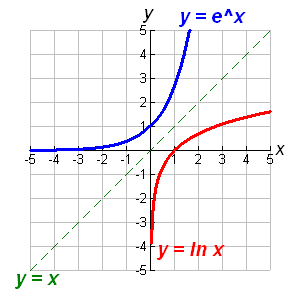
\includegraphics[scale=0.65]{images/003.png}
\begin{tikzpicture}
\draw[>=latex,<->,thick] (0,-1) -- (0,1) ;
\draw[>=latex,<->,thick] (-1,0) -- (1,0) ;
\node at (0,1.3) {N} ;
\node at (0,-1.3) {S} ;
\node at (1.3,0) {E} ;
\node at (-1.3,0) {O} ;

\draw[>=latex,->,thick] (4,0.75) -- (9,0.75) ;
\draw[>=latex,->,thick] (4.75,-1) -- (4.75,1.5) ;
\draw[thick] (5.75,0.75) arc (0:-22.5:1) ;
\node at (6,0.5) {$\alpha$} ;
\draw[->,thick] (4.75,0.75) -- (7.75,-0.5) node [near end, below] {$\vec{v}_{a/T}$};
\draw[->,thick,dashed] (7.75,-0.5) -- (7.75,0.75) node [midway, right] {$\vec{v}_{A/T}$} ;
\draw[->,thick] (4.75,0.75) -- (7.72,0.75) node [near end, above] {$\vec{v}_{a/A}$} ;

\end{tikzpicture}
\end{center}
On cherche $\vec{v}_{a/T}$ tel que $\vec{v}_{a/T}+\vec{v}_{A/T}=\vec{v}_{a/A}$ et $\alpha=(\vec{v}_{a/T};\vec{v}_{a/A})$.\\\\
On peut utiliser le théorème de Pythagore pour obtenir $||\vec{v}_{a/T}||$:\\\\
$||\vec{v}_{a/T}||=\sqrt{||\vec{v}_{a/A}||^{2}+||\vec{v}_{A/T}||^{2}}=\sqrt{50^{2}+120^{2}}=130km/h$.\\\\
Et $\alpha=Arctan(\frac{||\vec{v}_{A/T}||}{||\vec{v}_{a/A}||})=Arctan(\frac{50}{120})=22.6^{\circ}$.\\

\section{Forces et mouvement}
\subsection{Le principe fondamental de la dynamique}
La $2^{nde}$ loi de Newton établit que si l'on a un corps de masse m invariante, l'accélération subie par ce corps dans un référentiel galiléen est proportionnelle à la somme des forces qu'il subit et inversement proportionnelle a la masse.\\\\
$\sum\vec{F}_{ext}=m \vec{a}=\frac{d\vec{p}}{dt}$ (avec $\vec{p}=m\vec{v}$ la quantité de matière)\\

\subsubsection{Force}
Une force est une grandeur dont l'action sur un corps modifie la quantité de mouvement, ou encore une interaction entre deux systèmes à l'origine d'une accélération. Elle est représentée par un vecteur possédant une norme, une direction et un sens et sa valeur est exprimée en Newton (N) homogènes à des $kg*m*s^{-2}$.\\
La première définition montre que la quantité de mouvement d'un système isolé se conserve.\\

\subsubsection{Masse}
La grandeur masse est définie par Newton comme la résistance qu’un corps oppose à un effort extérieur. Il constate que pour un même effort, les objets se mettent plus ou moins "facilement" en mouvement (\textit{ie} leur accélération est plus ou moins grande).\\

\subsection{Équations horaires et de trajectoire}
L'objet de la dynamique est de décrire l’évolution de la position d'un système soumis à des forces extérieures au cours du temps. Il s'agit de chercher les équations paramétrées du mouvement (position en fonction du temps) ou l'équation de la trajectoire du système (y en fonction de x).\\

Pour déterminer ces équations, on fait le bilan des forces s'appliquant sur un système dans un référentiel précis pour en déduire l'accélération du système à l'aide du principe fondamental de la dynamique.\\
On peut ensuite en déduire la trajectoire du système si l'on connaît les conditions initiales.
\begin{center}
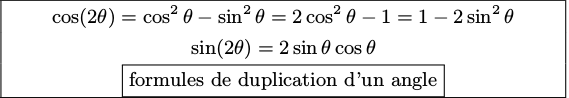
\includegraphics[scale=1.1]{images/012.png}
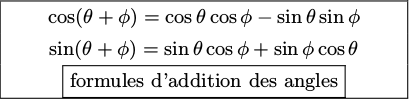
\includegraphics[width=15cm, height=18cm]{images/011.png}
\begin{large} $y(x)=-\frac{gx^{2}}{2v_{0}{}^{2}cos(\alpha)^{2}}+tan(\alpha)x$ $ $ $ $ $ $ $ $ $y(x)=-\frac{qEx^{2}}{2mv_{0}{}^{2}}$ \end{large}
\end{center}
\newpage

\subsection{Grandeurs cinématiques}
\subsubsection{Accélération} 
$\vec{a}(t)=\frac{d\vec{v}(t)}{dt}=\frac{d\overset{\longrightarrow}{OM}(t)}{dt^{2}}=\overset{.}{v}(t)\vec{i}+\overset{.}{v}(t)\vec{j}=\overset{..}{x}(t)\vec{i}+\overset{..}{y}(t)\vec{j}$\\

\subsubsection{Vitesse} 
$\vec{v}(t)=\displaystyle \int \vec{a}(t)dt=\frac{d\overset{\longrightarrow}{OM}(t)}{dt}$. En général, $||\vec{a}(t)||=c^{ste}$.\\

\subsubsection{Position} 
$\overset{\longrightarrow}{OM}(t)=\displaystyle \iint \vec{a}(t)dt=\displaystyle \int \vec{v}(t)dt$.\\\\

\subsubsection{Tracé de vecteur pour plusieurs situations}
\emph{Cas du mouvement parabolique}\\
Prenons une balle lancée avec une vitesse initiale $\vec{v}_{0}=\vec{v}_{0x}+\vec{v}_{0y}$ (les frottements avec l’air sont négligés) selon un angle à l'horizontale $\alpha$.\\
On constate ici que la composante horizontale de la vitesse initiale $v_{0x}$ reste inchangée tout au long du mouvement (pas d’accélération horizontale, pas de force horizontale appliquée sur la balle en mouvement donc le principe d’inertie s’applique horizontalement).\\
En revanche, la composante verticale de la vitesse initiale $v_{0y}$ varie tout au long du mouvement.
\begin{center}
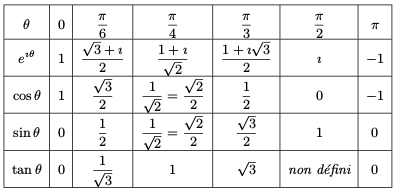
\includegraphics[scale=0.45]{images/007.png}
\end{center}

\emph{Cas du mouvement circulaire uniforme}\\
\begin{center}
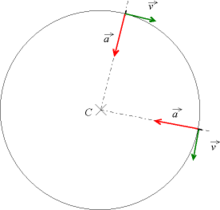
\includegraphics[scale=0.7]{images/006.png}
\end{center}


\subsection{Exemple de description cinématique du mouvement}
Une moto, au repos à un feu rouge, accélère uniformément dès que le feu passe au vert. Elle atteint ainsi une vitesse de $15 m*s^{-1}$ en 10s, vitesse qu’elle maintient pendant 30s. Elle freine ensuite uniformément pendant 5s pour s’immobiliser à un autre feu rouge.

\begin{center}\begin{tikzpicture}
\draw[>=latex,->] (-1,0) -- (11,0) ;
\node at (11.4,-0.2) {x(m)} ;
\node at (0,0) {|} ;
\node at (0,-0.4) {$t_{0}$} ;
\node at (2,0) {|} ;
\node at (2,-0.4) {$t_{1}$} ;
\node at (7,0) {|} ;
\node at (7,-0.4) {$t_{2}$} ;
\node at (9,0) {|} ;
\node at (9,-0.4) {$t_{3}$} ;
\node at (1,0.5) {(1)} ;
\node at (4.5,0.5) {(2)} ;
\node at (8,0.5) {(3)} ;
\draw[<->, thick] (0.1,1) -- (1.9,1) node[midway, above] {MRUA};
\draw[<->, thick] (2.1,1) -- (6.9,1) node[midway, above] {MRU};
\draw[<->, thick] (7.1,1) -- (8.9,1) node[midway, above] {MRUA};
\node at (-0.5,0.75) {feu} ;
\node at (-0.5,0.45) {rouge} ;
\node at (-0.5,0.2) {n$^{\circ}$1} ;
\node at (9.5,0.75) {feu} ;
\node at (9.5,0.45) {rouge} ;
\node at (9.5,0.2) {n$^{\circ}$2} ;
\node at (1,-1) {$a_{1}=c^{ste}$} ;
\node at (1,-1.5) {$t_{1}-t_{0}=10$s} ;
\node at (4.5,-1) {$v_{2}=15$m$\cdot$s$^{-1}$} ;
\node at (4.5,-1.5) {$t_{2}-t_{1}=30$s} ;
\node at (8,-1) {$a_{3}=c^{ste}$} ;
\node at (8,-1.5) {$t_{3}-t_{2}=5$s} ;
\end{tikzpicture} \end{center}

1) distance parcourue en (1) ?

2) distance parcourue en (2) ?

3) distance parcourue en (3) ?\\

En prenant pour système la moto et pour référentiel le référentiel terrestre supposé Galiléen, ayant pour origine spatiale la position initiale de la moto et pour origine temporelle $t_{0}$, on obtient\\\\
comme conditions initiales:$\left \{ \begin{array}{rcl} OM_{x}(t_{0})&=&0 \\
v_{x}(t_{0})&=&0 \\
a_{x}(t_{0})&=&a_{1} \\ \end{array} \right . $\\\\

En (1), on a une accélération constante et une vitesse initiale nulle, on obtient donc que l'équation horaire de la vitesse est $v(t)=a_{1}t$ or à ($t=10s$), on sait que $v(10)=15m/s$ donc on en déduit que $a_{1}=\frac{v(t)}{t}=\frac{15}{10}=1.5m*s^{-2}$.\\\\
On obtient ainsi que l'équation horaire de la position est $x(t)=\frac{1}{2}a_{1}t^{2}$. Ainsi, en $t_{1}$, la moto a parcouru $d_{10}=x(10)=\frac{1}{2}*1.5*10^{2}=75m$.\\

En (2), on a une vitesse constante sur $t_{2}-t_{1}=30s$ et donc $d_{2}=v_{1}*(t_{2}-t_{1})=15*30=450m$.\\

Enfin, en (3), (en prenant pour nouvelles origines des temps et de la position $t_{3}$ et la position de la moto à $t_{3}$) on a une vitesse initiale $v_{2}=15m/s$ et une accélération $a_{3}$ négative constante.\\\\
On obtient donc l'équation horaire de la vitesse : $v(t)=a_{3}t+v_{2}$, or à ($t=5s$), la moto est à l’arrêt donc $v(5)=0$ d'où $a_{3}=-\frac{v_{2}}{t}=-\frac{15}{5}=-3$ $m*s^{-2}$.\\\\
On obtient ainsi que l'équation horaire de la position est $x(t)=\frac{1}{2}a_{3}t^{2}+v{2}t$.\\\\ Ainsi, entre $t_{2}$ et $t_{3}$, la moto a parcouru $d_{3}=x(5)=-\frac{1}{2}*3*5^{2}=37.5m$.\\\\

La moto a donc parcouru en tout et pour tout $d=d_{1}+d_{2}+d_{3}=75+450+37.5=562.5m$.

\section{Représentation graphique des grandeurs cinématiques}

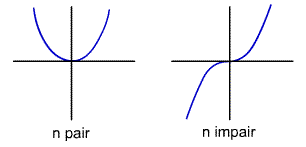
\includegraphics[scale=0.6]{images/008.png}
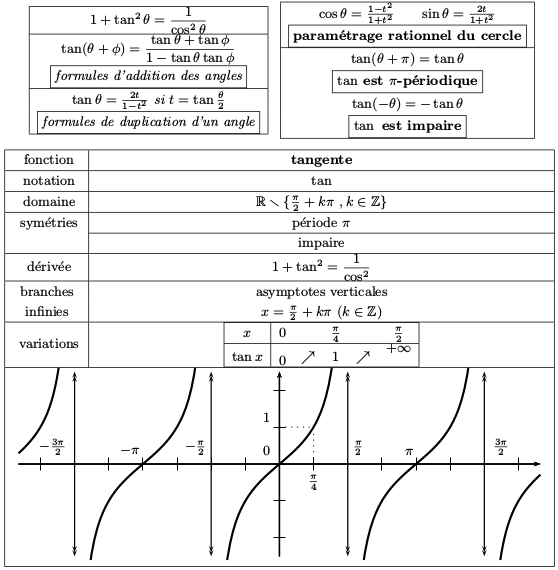
\includegraphics[scale=0.47]{images/009.png}

Le premier schéma montre la représentation graphique des grandeurs cinématiques dans le cas d'un mouvement uniforme et le deuxième dans le cas d'un mouvement uniformément accéléré.

\section{Systèmes en interaction : 3$^{e}$ loi de Newton}
La loi des actions réciproques établit que tout corps A exerçant une force sur un corps B subit une force d'intensité égale, de même direction, mais de sens opposé à celle exercée sur le corps B.
\begin{wrapfigure}[14]{r}{4.5cm}
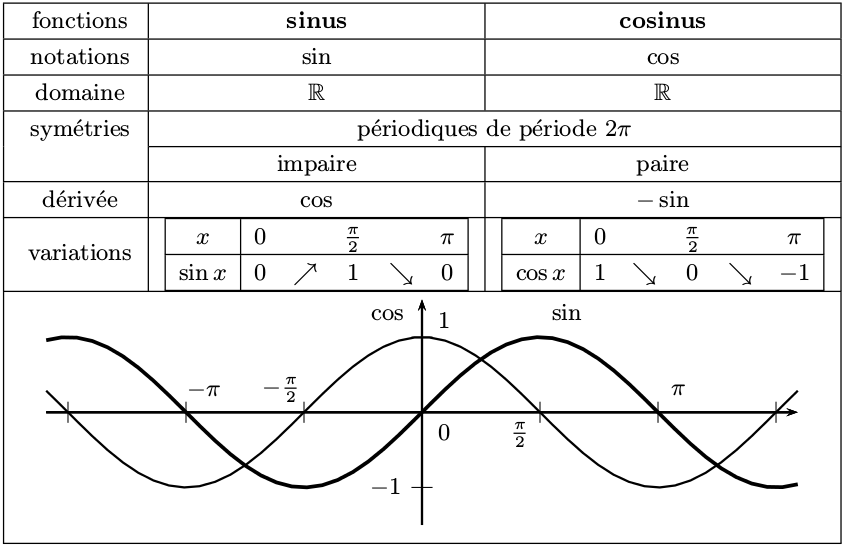
\includegraphics[scale=0.8]{images/010.png}
\end{wrapfigure}

\subsection*{Exemple}

Prenons l'exemple d'un clou que l'on enfonce dans une planche avec un marteau.\\
3 systèmes en interaction : planche, clou et marteau.\\

On s’intéresse au système \{clou\}.\\
Ce système est en interaction avec le marteau et la planche. La résultante des forces appliquées sur le clou est non nulle et dirigée vers la planche. Le clou s'enfonce dans la planche non pas parce que la force exercé par celui-ci sur la planche est plus importante que la résistance de la planche mais parce que la force exercée par le marteau sur le clou est plus grande que celle exercée par la planche sur le clou (la force du marteau est transmise à la planche).

\chapter{Forces et interactions}
\section{Champ, interaction et concept de force}
\subsection*{Définition}
En physique, un champ est la donnée, pour chaque point de l’espace-temps, de la valeur d’une grandeur physique. La source d’un champ peut être une masse, une charge, etc. Une masse (une charge) placée dans un champ est en interaction avec la source du champ.

\section{Force de gravité}
\subsection{Définition}
La force de gravité est le force qui modélise l’interaction gravitationnelle. Un objet de masse m génère autour de lui un champ que l’on peut définir comme la modification de la propriété gravitationnelle de l’espace. Un objet de masse m placé dans ce champ est soumis à la force exercée par m.

\subsection{Formule}
$F_{a/b}=G$ $\frac{mm'}{r^{2}}$ $\vec{u}$ $ $ $ $ avec m et m' les masses en interaction, r la distance entre a et b et $G=-6.67\times 10^{-11} N\times m^{2}\times kg^{-2}$.\\\\
D'après la troisième loi de Newton, $\vec{F}_{b/a}=-\vec{F}_{a/b}$.\\

\subsubsection{Cas particulier}
\emph{Force de gravité au voisinage de la Terre}\\

$\vec{P}=m\vec{g}$\\\\
Le poids $\vec{P}=m\vec{g}$ est un cas particulier de la force de gravité ramenée à la surface de la Terre\\
d'où $g=G$ $\frac{M_{T}}{R_{T}{}^{2}}$ $ $avec $M_{T}=6*10^{24} kg$ la masse de la Terre et $R_{T}=6400 km$ la rayon de la Terre.\\

\textit{Newton unifie le sublunaire et le supralunaire en montrant que la cause de la chute des corps sur Terre est la même que celle qui "retient" la Lune en orbite autour de la Terre.}

\newpage

\subsection{Étude d'un mouvement dans le champ de pesanteur terrestre}
On lance un projectile avec une vitesse initiale $\vec{v_{0}}$ à une hauteur h selon un angle $\alpha$. On étudie le mouvement dans le référentiel Terrestre supposé galiléen.\\

Le système est le projectile de masse m et l'origine du repère orthogonal est telle que l'axe $O_{x}$ est dans le sens de $v_{0}$ et telle que $O_{z}$ est du sol vers la position à $t_{0}$ du projectile.\\

On fait l'inventaire des forces extérieures, il n'y a que le poids.\\
On projette sur les axes $O_{x}$ et $O_{z}$:\\\\
$x(t)=v_{0}cos(\alpha)t$\\
$z(t)=-0.5gt^{2}+v_{0}sin(\alpha)t+h$\\\\
donc $z(x)=-\frac{0.5gx^{2}}{v_{0}{}^{2}cos^{2}(\alpha)}+x*tan(\alpha)+h$.\\\\

\section{Force électrostatique - champ électrique}
\begin{center} \begin{Large}
$\vec{F}_{1/2}=\frac{q_{1}q_{2}}{4\pi \epsilon r^{2}}\vec{u}$\\ \end{Large} \end{center}

$\vec{F}$ est la force exercée par une charge $q_{1}$ sur une charge $q_{2}$ avec $\epsilon$ la permittivité du milieu, et r la distance entre les deux charges électriques.\\

$q_{2}$ "subit" le champ électrique $E_{1/2}$ généré par $q_{1}$ (et réciproquement) tel que $E_{1/2}=\frac{q_{1}}{4\pi \epsilon r^{2}}$. On a donc $\vec{F}_{1/2}=q_{2}\vec{E}_{1/2}$.\\

Pour une charge q entre deux plaques d’un condensateur au sein duquel règne un champ électrique uniforme $E$ $:$ $F=qE$.\\

Ces forces sont à l’origine des forces de frottement.\\\\\\

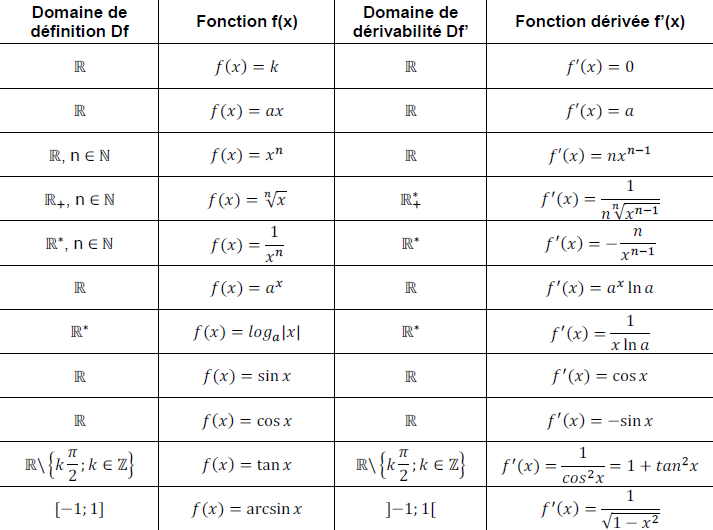
\includegraphics[scale=1]{images/017.png}

\newpage

\section{Forces de contact}
\subsection{Forces de contact solide}
Dans le référentiel galiléen associé à la table le système \{solide S\} est immobile, alors \begin{wrapfigure}[12]{r}{6cm} 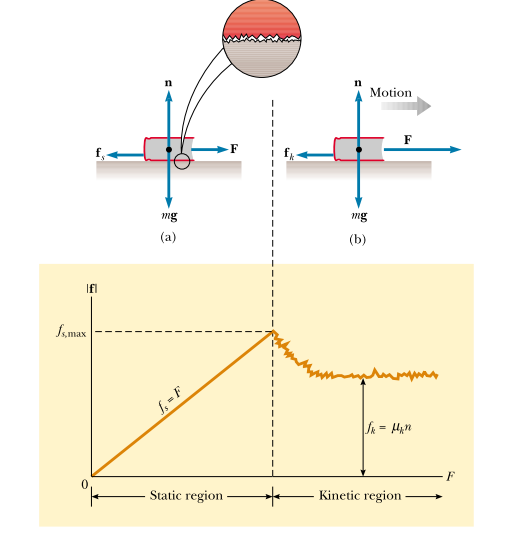
\includegraphics[scale=0.42]{images/014.png} \end{wrapfigure}
$\begin{array}{rcl} \sum \vec{F}_{ext}=\vec{0} &\Leftrightarrow & \vec{P}+\vec{R}=\vec{0}\\
&\Leftrightarrow & ||\vec{P}||=||\vec{R}|| \text{ et } \vec{P}=-\vec{R} \end{array}$\\\\

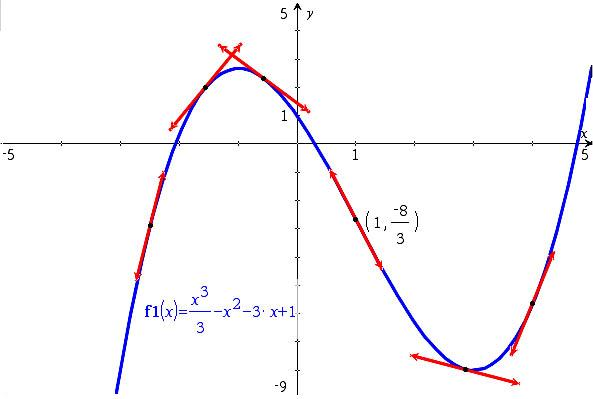
\includegraphics[scale=0.75]{images/016.png}

Supposons qu'un opérateur tire l'objet vers la droite.

\subsubsection{1$^{er}$ cas : régime statique}
L'objet reste au repos donc $\sum\vec{F}_{ext}=\vec{0}\\
\Leftrightarrow \vec{P}+\vec{N}+\vec{F}_{opérateur/objet}+\vec{F}_{table/objet}=\vec{0}\\
\Leftrightarrow \vec{F}_{opérateur/objet}=-\vec{F}_{table/objet}$\\

($\vec{F}_{table/objet}=\vec{F}_{s}$ est la force de frottement statique, sa direction est celle du mouvement)\\

Dans ce cas (statique), il existe une relation entre $\vec{F}_{s}$ et $\vec{N}$ : $||F_{s}|| < \mu_{s}*||\vec{N}||$ ($\mu_{s}$ est le coefficient de frottement statique).

\subsubsection{2$^{eme}$ cas : régime dynamique ou cinétique}
L'objet se met en mouvement donc $\sum \vec{F}_{ext}=m\vec{a}\neq \vec{0}$ (m masse constante de l'objet)\\

$\vec{P}+\vec{N}+\vec{F}_{opérateur/objet}+\vec{F}_{table/objet} = m\vec{a}\neq 0$\\

Dans ce cas (dynamique), il existe aussi une relation entre $||\vec{F}_{d}||$ et $||\vec{N}||$:\\
$||\vec{F}_{d}||=\mu_{d}||\vec{N}||$ (au moment où l'objet se met en mouvement, $\mu_{d}$ est le coefficient de\\ frottement dynamique).\\

Il faut noter que les coefficients statique et dynamique dépendent de la nature des surfaces en contact.\\

\emph{Application :} trouver la valeur de l'angle $\phi$ en fonction de $\mu_{d}$ pour qu'il y ait un glissement
\begin{center} 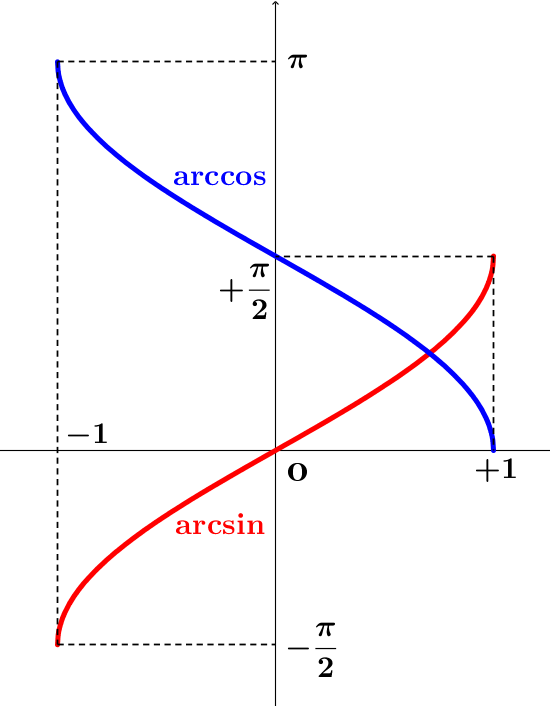
\includegraphics[scale=0.6]{images/015.jpg}

$\phi >Arctan(\mu_{d})$ \end{center}


\subsection{Forces de contact solide-fluide}
Un frottement fluide est une force de frottement qui s’exerce sur un objet qui se déplace dans un fluide ; elle dépend de la vitesse relative de l’objet et du fluide. Comme toutes les forces de frottement, cette force dépend fortement de la géométrie de l’objet considéré, de sa surface.\\

\subsubsection{Concept de pression}
La pression en un point d’un fluide de masse volumique $\rho_{fluide}$ est dépendante uniquement de la hauteur de fluide au-dessus du point considéré.\\

A titre d’exemple, la pression au-dessus du cube de volume $V_{cube}$ immergé est inférieure à la pression au-dessous. Cette différence de pression est à l’origine de la poussée d’Archimède (désignée sur la figure par la lettre B) ; cette force est la résultante (ie :la somme) de l’ensemble des forces pressantes exercées par le fluide sur le cube, sachant qu’une force pressante est le produit de la pression en un point du fluide par la surface de l’objet sur laquelle elle s’exerce.\\

La poussée d’Archimède est dans la même direction et dans le sens opposé à la force exercée par la Terre sur l’objet immergé (désignée $\vec{F}_{g}$ sur la figure) et sa norme est $B=\rho_{fluide}\times g\times V_{cube}$ (cette force correspond en fait au poids $\vec{P}$ du volume de liquide déplacé par l'objet, ce volume étant donc celui de l'objet plongé).\\

\begin{center} 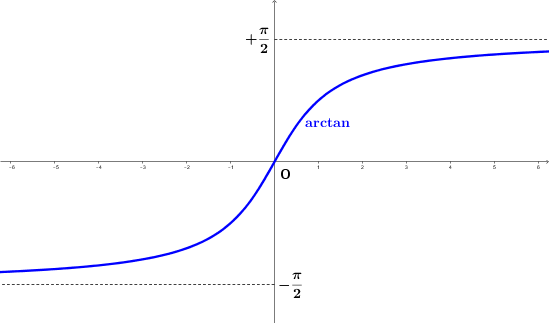
\includegraphics[scale=1.15]{images/018.png} \end{center}
\newpage

\begin{wrapfigure}[4]{r}{2cm} 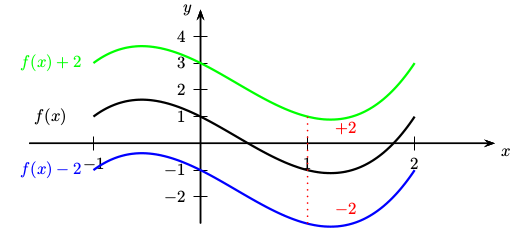
\includegraphics[scale=0.6]{images/019.png} \end{wrapfigure}
Tous les liquides ne s’écoulent pas de la même manière. On distingue deux régimes d’écoulement, les écoulement laminaires et les écoulements turbulents qui se distinguent par exemple par le comportement d’un fluide s’écoulant autour d’un obstacle.


\subsubsection{Cas 1 : régime laminaire}
Ce cas concerne les objets de faible volume en mouvement à basse vitesse\\ ($5$ $m/s$) dans un fluide plutôt visqueux.\\\\
Dans ce cas, la force de frottement fluide a pour expression $\vec{f}=-k\vec{v}$\\
avec $k=6\pi\eta r$ pour une sphère de rayon r et $\eta$ le coefficient de viscosité.\\

La vitesse limite constante est égale à $v_{lim}=\frac{\rho Vg-mg}{k}$.

\begin{wrapfigure}[2]{r}{2cm} 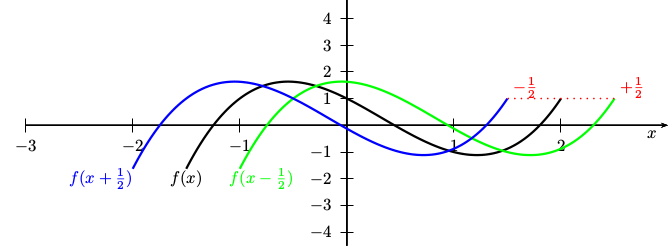
\includegraphics[scale=0.6]{images/020.png} \end{wrapfigure}

\subsubsection{Cas 2 : régime turbulent}
Dans ce cas, la force de frottement fluide a pour expression $\vec{f}=-\frac{1}{2}C\rho S v^{2}\frac{\vec{v}}{v}$\\
avec $\rho$ la masse volumique des fluides, S l'aire du solide selon la direction perpendiculaire à la vitesse et C le coefficient de traînée caractérisant le solide.\\\\\\\\

\subsubsection{Nombre de Reynolds}
La frontière entre ces deux situations est assez mince, et on peut la percevoir au moyen d’une quantité appelée nombre de Reynolds $R_{e}$.\\

Il permet de détecter l’apparition de la turbulence : plus il est élevé, plus la vitesse d’écoulement est importante et la viscosité faible, et plus les tourbillons pourront se développer.\\

\begin{wrapfigure}[10]{l}{3cm}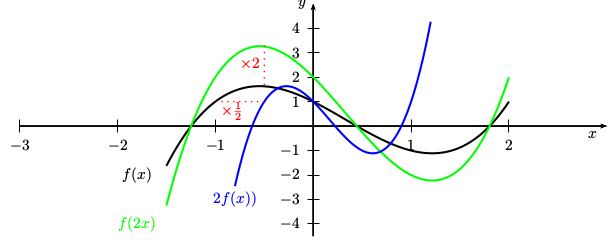
\includegraphics[scale=0.23]{images/021.png} \end{wrapfigure}$\text{\\}$

On peut dire que la viscosité $\eta$ rend compte de la capacité d’un fluide de masse volumique $\rho$ à s’écouler (ie : la résistance d’un fluide à l’écoulement sans turbulence).\\

Les forces de viscosité sont d’autant plus importantes que la viscosité $\eta$ du fluide est élevée, que sa vitesse v est importante, et que le diamètre L de l’écoulement est petit.\\

Le nombre de Reynolds de l’écoulement est tel que : $R_{e}=\frac{v\rho L}{\eta}$.\\\\

Si $R_{e}\ll 1$, il s'agit d'un régime laminaire, si $R_{e}>2000$ alors c'est un régime turbulent ; entre les deux il est difficile de déterminer ce qui se passe.\\\\
Un exemple classique de transition laminaire / turbulent est celui de la dissipation de la vapeur d’eau (voir photo ci-contre).

\newpage

\subsection{Application dans un régime laminaire}
\subsubsection{Résolution de l’équation différentielle}
On prend le cas de la chute d'une balle dans un fluide visqueux (glycérine/huile) donc d'un régime laminaire.\\

Le système est la \{bille de masse m\} dans un référentiel attaché a la terre et considéré comme galiléen.
On fait l'inventaire des forces extérieures : \begin{itemize}\renewcommand{\labelitemi}{$\bullet$}
\item poids $\vec{P}=-mg*\vec{k}$
\item frottement $\vec{f}=-kv*\vec{k}$
\item poussée d'Archimède $\vec{A}=\rho Vg*\vec{k}$\\ \end{itemize}

D'après le PFD : $\sum \vec{F}=m\vec{a}=\vec{P}+\vec{f}+\vec{A}$ donc $\frac{dv}{dt}+\frac{kv}{m}=\frac{\rho Vg}{m}-g$.\\

On va résoudre l'équation différentielle du premier ordre sans second membre:\\
Pour cela il faut trouver une solution particulière que l'on va ajouter à la solution de cette équation sans le second membre.\\

On détermine une solution particulière :\\
On choisit une valeur de v constante, on a donc $\frac{dv}{dt}=0$ donc $\frac{kv}{m}=\frac{\rho Vg}{m}-g$ d'où $v=\frac{\rho Vg-mg}{k}$.\\
On appelle ce v la vitesse limite car il s'agit de la vitesse théorique maximale atteinte par le système à l'infini.\\

On résout maintenant l'équation différentielle sans second membre (en prenant v comme une valeur algébrique):\\

$\begin{array}{rcl}\frac{dv}{dt}+\frac{kv}{m}=0 &\Leftrightarrow& \frac{dv}{dt}=-\frac{kv}{m} \\\\
&\Leftrightarrow& \frac{dv}{v}=-\frac{k}{m}dt \\\\
&\Leftrightarrow& \displaystyle \int_{v} \frac{dv}{v}=\displaystyle \int_{t} -\frac{k}{m}dt \\\\
&\Leftrightarrow& ln(v)=-\frac{k}{m}t+C \text{ avec C une constante}\\\\
&\Leftrightarrow& v=C' e^{-\frac{k}{m}t} \text{ avec } C'=e^{C} \text{ une constante} \\\\ \end{array} $

On utilise maintenant les conditions initiales pour trouver C' :\\
on sait que $v(0)=0$ donc on a $v(0)=C'+v_{lim}=0$ d'où $C'=-v_{lim}$.\\

On a donc $v(t)=\frac{\rho Vg-mg}{k}(1-e^{-\frac{k}{m}t})$.\\

On appelle temps caractéristique $\tau =\frac{m}{k}$, on a alors que la vitesse limite est atteinte (on la considère atteinte quand $v=0.99*v_{lim}$) en $t=5\tau$.\\
De plus, $\tau$ est l'abscisse du point d'intersection de la tangente à l'origine et de la droite horizontale d'équation $y=v_{lim}$.

\begin{center} 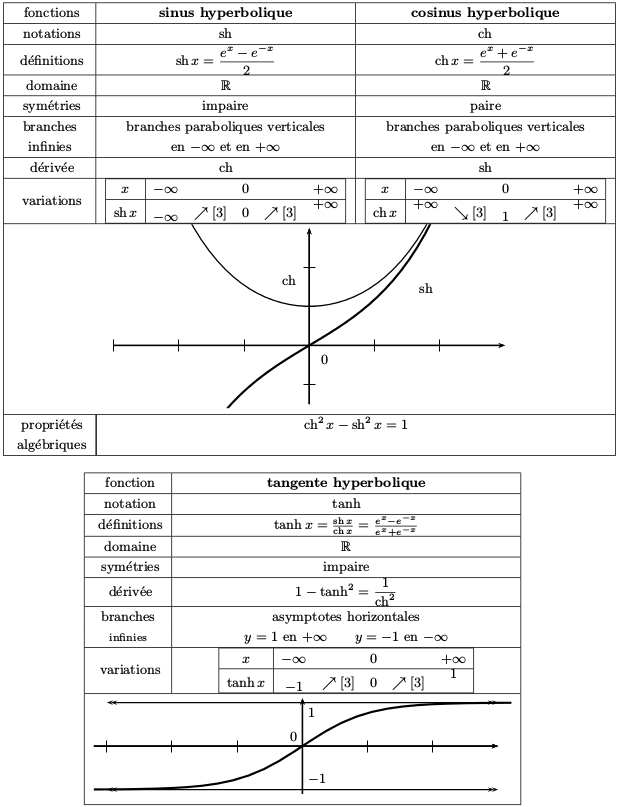
\includegraphics[scale=0.55]{images/022.png} \end{center}

\chapter{Énergie}
\section{Définition}
\emph{"L’énergie nous apparaît sous un très grand nombre de formes différentes, et il existe une formule pour chacune. Ce sont : l’énergie gravitationnelle, l’énergie cinétique, l’énergie thermique, l’énergie élastique, l’énergie électrique, l’énergie chimique, l’énergie de rayonnement, l’énergie nucléaire, l’énergie de masse. Il est important de se rendre compte que dans la physique d’aujourd’hui, nous n’avons aucune connaissance de ce qu’est l’énergie".} \textbf{Richard Feynman}\\

On peut toutefois tenter une définition du type "l’énergie est une notion qui quantifie la capacité d’un système à se transformer - à changer d’état". Il s’agit
\begin{itemize}\renewcommand{\labelitemi}{$\bullet$} \item d’un concept de type "formel" qui n’a pas de correspondant dans le monde sensible ;
\item d’une grandeur que l’on associe à un objet (un système) pour qualifier l’état dans lequel il se trouve (conséquence : si l’état change, la valeur de la grandeur change).\\ \end{itemize}

A noter, l’unité de l’énergie est le Joule J (qui représente par exemple l’énergie requise pour élever une pomme (100 grammes) d’un mètre dans le champ de pesanteur terrestre mais également l’énergie nécessaire pour élever la température d’un gramme (un litre) d’air sec d’un degré Celsius).


\section{Énergie cinétique et travail}
\subsubsection{Définition}
Le travail est la capacité d'une force à changer l'état énergétique d'un système (en particulier l'énergie cinétique mais pas uniquement).
\subsection{Travail d'une force constante}
On restreint l’étude du concept de travail à des situations relevant de la dynamique newtonienne, c’est à dire, à la capacité des forces à modifier l’énergie de type "mécanique" des systèmes. Nous nous intéressons donc aux travaux des forces qui provoquent le déplacement (spatial) des systèmes à l’étude.\\

Formellement, le travail W d’une force constante $\vec{F}$ est le produit scalaire de la force exercée sur un système par le déplacement $\Delta\vec{x}$ effectué par ce système pendant toute la durée de l’application de la force, avec $\Delta\vec{x}= (x_{f}-x_{i})\vec{i}$. (Ici, on considère un système en déplacement le long d’un axe $(O_{x})$, auquel on associé un vecteur unitaire $\vec{i}$ avec $x_{f}=$ position finale et $x_{i}=$ position initiale).

\begin{center} $W=\vec{F}\cdot\Delta\vec{x}$ \end{center}

\subsection{Travail d'une force variable}
Si la force qui s’applique à un système n’est pas constante (par exemple, la force de rappel d’un ressort, ou la force de gravité) on ne peut plus appliquer la formule précédente. En revanche, on peut prendre un tout petit déplacement $\Delta_{x}$ et considérer que sur ce petit déplacement, la composante selon x de la force $F_{x}$ appliquée sur le système est constante. Le travail de la force s’écrit alors :
\begin{center} $\Delta W=\vec{F}_{x}\cdot\Delta \vec{x}$\\ \end{center}

\begin{center} $W_{x_{i}\rightarrow x_{f}}=\displaystyle\int_{x_{i}}^{x_{f}}\vec{F}_{x}$ $d\vec{x}$\\ \end{center}

\begin{center} 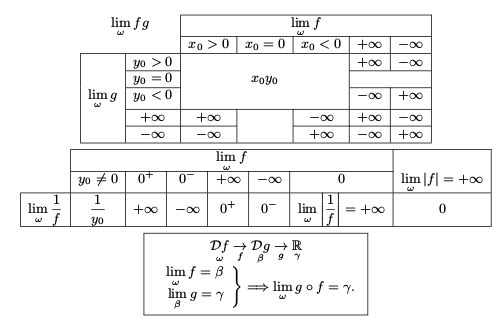
\includegraphics[scale=0.4]{images/023.png} \end{center}

Le travail \textbf{W} de la composante selon x de la force exercée sur un système le long d’un petit déplacement est égal au produit scalaire de la force par ce petit déplacement (rectangle coloré sur la figure). Le travail total de la force sur l’ensemble du déplacement est la somme de tous les rectangles sous la courbe représentant la variation de la composante selon x de la force exercée sur le système en déplacement.\\

\subsubsection{Exemple du travail de la force de gravité}
La force de gravité est exercée par un corps A de masse M sur un corps B de masse m dont les centres de gravité sont espacés d’une distance r :\\
\begin{center} $\vec{F}_{g}=-G\frac{mM}{r^{2}}\vec{u}_{r}$ \end{center}

Avec $\vec{u}_{r}=\overrightarrow{AB}$. Le travail de la force de gravité pour un changement de position du corps B d’une distance $r_{1}$ à une distance $r_{2}$ s’exprime de la manière suivante :\\

\begin{center} $\begin{array}{rcl}
W_{r_{1}\rightarrow r_{2}}&=& \displaystyle \int_{r_{1}}^{r_{2}}\vec{F}_{g}\cdot d\vec{r}\\\\
W_{r_{1}\rightarrow r_{2}}&=& \displaystyle \int_{r_{1}}^{r_{2}}F_{g}*\vec{u}_{r}\cdot dr*\vec{u}_{r}\\\\
W_{r_{1}\rightarrow r_{2}}&=& -GMm\displaystyle \int_{r_{1}}^{r_{2}}\frac{1}{r^{2}}dr \\\\
W_{r_{1}\rightarrow r_{2}}&=& -GMm\displaystyle \left[ -\frac{1}{r} \right]_{r_{1}}^{r_{2}}=-GMm(\displaystyle \frac{1}{r_{1}}-\frac{1}{r_{2}})\\\\
\end{array}$ \end{center}

On constate que si on éloigne le corps B du corps A alors le travail de la force de gravité exercée par A sur B est négatif (travail résistant). Au contraire si on approche le corps B du corps A alors le travail de la force de gravité exercée par A sur B est positif (travail moteur).

\section{Théorème de l'énergie cinétique}
\subsection{Énoncé}
On a démontré dans le cours que la somme des travaux des forces qui s’appliquent sur un système modifie l’état cinétique de ce système. Formellement, la somme des travaux des forces qui s’appliquent sur un système est égale à la variation d’énergie cinétique de ce système :
\begin{center} $\sum W_{\text{F. ext}}=\Delta E_{c}$ \end{center}
Avec $\Delta E_{c}=E_{c_{f}}-E_{c_{i}}=\frac{1}{2}mv^{2}_{f}-\frac{1}{2}mv^{2}_{i}$.\\

\subsubsection{Propriété}
On sait que $W_{\vec{F}}=\displaystyle \int_{x_{i}}^{x_{f}} \vec{F}\cdot d\vec{x}$.\\

Mais de plus, dans le cas où plusieurs forces s'exercent sur un système,\\
on a $W_{\sum\vec{F}_{ext}}=\displaystyle \int_{x_{i}}^{x_{f}} \sum \vec{F}\cdot d\vec{x}$.\\

\subsection{Démonstration du théorème}
On veut montrer que $W_{\sum\vec{F}_{ext}}=\Delta E_{c}$ :\\\\

$\begin{array}{rcl} W_{\sum\vec{F}_{ext}}&=&\displaystyle \int_{x_{i}}^{x_{f}} \sum \vec{F}\cdot\vec{dx}\, \text{ donc d'après le PFD on a}\\\\
&=&\displaystyle \int_{x_{i}}^{x_{f}} m\vec{a}\cdot\vec{dx}\, \text{ or }\vec{a}=\frac{d\vec{v}}{dt} donc\\\\
&=&\displaystyle \int_{x_{i}}^{x_{f}} m\frac{d\vec{v}}{dt}\cdot\vec{dx}\\\\
&=&\displaystyle \int_{x_{i}}^{x_{f}} m\frac{d\vec{x}}{dt}\cdot d\vec{v}\, \text{ or }\frac{d\vec{x}}{dt}=\vec{v} \text{ donc}\\\\
&=&\displaystyle \int_{v_{i}}^{v_{f}} m\vec{v}\cdot d\vec{v}\, \text{ d'où}\\\\
&=&\displaystyle \int_{v_{i}}^{v_{f}} mv \, dv\\\\
&=&\left[ \frac{1}{2}mv^{2} \right]_{v_{i}}^{v_{f}}=\frac{1}{2}mv_{f}{}^{2}-\frac{1}{2}mv_{i}{}^{2}\\\\
W_{\sum\vec{F}_{ext}}&=&\Delta E_{c}\\\\\\\\\\\\ \end{array}$

\subsection{Application}

Donner l'expression du travail des forces appliquées sur un bloc glissant avec frottement sur un plan incliné de longueur l avec un angle $\phi$ par rapport à l'horizontale.\\
\begin{center} 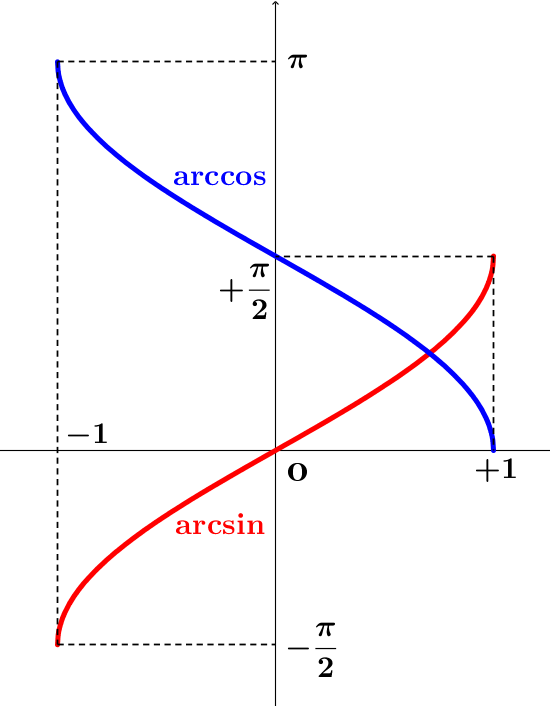
\includegraphics[scale=0.35]{images/015.jpg} \end{center}

$W_{\vec{P}}=\vec{P}\cdot\vec{l}=m*g*l*cos((\vec{P};\vec{l}))=mgl*cos(\beta)$ avec $\beta=\frac{\pi}{2}-\phi$\\
donc $cos(\beta)=sin(\phi)$ d'où $W_{\vec{P}}=mgl*sin(\phi)$\\

$W_{\vec{R}_{N}}=R_{N}*l*cos((\vec{R}_{N};\vec{l}))=0$\\

$W_{\vec{R}_{T}}=R_{T}*l*cos((\vec{R}_{T};\vec{l}))=R_{T}*l*cos(\pi)=-R_{T}*l$

\section{Énergie potentielle et force conservative}
\subsection{Énergie potentielle}
\subsubsection{Définition}
L'énergie potentielle rend compte de l'organisation de plusieurs systèmes en interaction les uns avec les autres. 

\subsection{Force conservative}
\subsubsection{Définition}
Une force conservative est une force dont le travail ne dépend pas du chemin suivi par un système sur lequel cette force s'applique.

\begin{figure}[h] \begin{center} 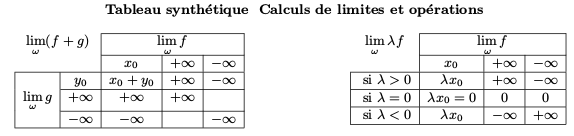
\includegraphics[scale=0.25]{images/024.png}
\caption{Peu importe le chemin pris, le travail d'une force conservative est le même}\end{center} \end{figure}

Dans le cas où $\vec{F}$ est conservative, on a $\vec{F}=\overrightarrow{\mathcal{G}\text{rad}}\, Ep$. Selon la dimension $\vec{i}$, $\vec{F}$ s'écrit $\vec{F}=-\frac{dEp}{dx}\vec{i}$. Conservatif ne veut pas dire constant.\\

Les forces centrales sont conservatives.

\subsubsection{Exemples}
\begin{itemize}\renewcommand{\labelitemi}{$\bullet$}
\item Force de gravité.
\item Force de Coulomb.
\item Force de rappel d'un ressort.\\
\end{itemize}

En revanche, les forces de frottement ne sont pas conservatives.

\subsection{Travail d'une force conservative}
$\begin{array}{rcl} \vec{F}=-\frac{dEp}{dx}\vec{i} &\Leftrightarrow & F=-\frac{dEp}{dx}\\\\
&\Leftrightarrow &F\, dx=-d\, Ep\\\\
&\Leftrightarrow &\displaystyle \int_{x} F\, dx=-\int_{Ep_{i}}^{Ep_{f}}dEp\\\\
&\Leftrightarrow &\displaystyle \int_{x} F\, dx=- \left[ Ep \right] {}_{Ep_{i}}^{Ep_{f}}=-(Ep_{f}-Ep_{i})\\\\ \end{array}$

Donc $W_{\vec{F}_{x_{i}\rightarrow x_{f}}}=-\Delta Ep$.

\section{Énergie mécanique}
\subsection{Conservation de l'énergie mécanique}
Dans le cas de systèmes conservatifs, (c'est-à-dire soumis à des forces conservatives),
\begin{center} $W_{\vec{F}}=-\Delta Ep$ et $W_{\vec{F}}=\Delta Ec$ \end{center}

\emph{Conséquence :} Dans le cas des systèmes conservatifs on a $-\Delta Ep=\Delta Ec \Leftrightarrow \Delta Ep+\Delta Ec=0$.\\

Lorsqu'un système est soumis à des forces conservatives, l'énergie mécanique totale du système (somme de l'énergie cinétique et de l'énergie potentielle) ne varie pas au cours du temps, on dit que l'énergie mécanique se conserve.

\subsection{Application}
\textit{Travail de la force de gravité entre deux positions A et B par la trajectoire (b)}

\begin{center} \begin{tikzpicture}[scale=0.95]
\draw (0,0) circle (0.75) ;
\node at (0.7,-0.8) {(M)} ;
\node at (0,0) {$\times$} ;
\node at (-0.2,-0.2) {O} ;
\draw (0,0) -- (3,0) ;
\node at (3,-0.3) {A'} ;
\node at (3,0) {$\bullet$} ;
\draw (3,0) arc (0:20:3) ;
\draw[>=latex,->] (3,0) -- (6.5,0) ;
\node at (5,0) {$\bullet$} ;
\node at (5,-0.3) {B} ;
\node at (2.81,1.02) {$\bullet$} ;
\draw (0,0) -- (2.81,1.02) ;
\node at (2.81,1.32) {A} ;
\draw[->,thick] (2.81,1.02) -- (1.8,0.655) node[near end, above] {$\vec{F}$} ;
\draw[->,thick] (3,0) -- (1.89,0) node[near end, above] {$\vec{F}$} ;
\draw[->,thick] (2.81,1.02) arc (20:15:3) ;
\node at (3.15,1) {d$\vec{v}$} ;
\draw[->,thick] (3,0) -- (3.325,0) node[above, near end] {d$\vec{r}$} ;
\draw (2.81,1.02) arc (130:50:1) ;
\draw (4.095,1.02) arc (-130:-90:1) ;
\draw (5,0) arc (-50:87:0.4445) ;
\node at (4.5,1.15) {(b)} ;
\draw[->,thick] (5,0) -- (5.5,0) node[above right, midway] {$\vec{u}_{r}$} ;
\end{tikzpicture} \end{center}

La force de gravité est conservative donc on peut étudier son travail sur le trajet A-A'-B, ce qui est plus pratique puisque sur A-A', la force de gravité est perpendiculaire à la trajectoire (donc son travail est nul).\\

Ainsi entre les deux points A et B : $W_{\vec{F}_{A\rightarrow B}}=W_{\vec{F}_{A\rightarrow A'}}+W_{\vec{F}_{A'\rightarrow B}}=W_{\vec{F}_{A'\rightarrow B}}$

On appelle $OA'=r_{1}$ et $OB=r_{2}$, on cherche $W_{\vec{F}_{r_{1}\rightarrow r_{2}}}$:\\

$\begin{array}{rcl} W_{\vec{F}_{r_{1}\rightarrow r_{2}}}&=&\displaystyle \int_{r_{1}}^{r_{2}}\vec{F}\cdot d\vec{r} \text{ avec } \vec{F}=-\mathcal{G}\frac{Mm}{r^{2}}\vec{u}_{r}\\\\
&=& \displaystyle \int_{r_{1}}^{r_{2}}-\mathcal{G}\frac{Mm}{r^{2}}\vec{u}_{r}\cdot dr\vec{u}_{r}\\\\
&=& \displaystyle \int_{r_{1}}^{r_{2}}-\mathcal{G}\frac{Mm}{r^{2}}\,dr\\\\
&=& \mathcal{G}Mm \left[ \frac{1}{r} \right]_{r_{1}}^{r_{2}}\\\\
W_{\vec{F}_{r_{1}\rightarrow r_{2}}} &=& \mathcal{G}Mm(\frac{1}{r_{2}}-\frac{1}{r_{1}}) <0 \text{ (travail résistant)}\end{array}$\\

\subsubsection{Vitesse de libération}
\emph{Définition :} La vitesse de libération est la vitesse à fournir à un système à la surface de la terre pour que son énergie mécanique à l'infini soit nulle.\\\\

\textit{Calcul :}\\\\
La force de gravité est conservative donc $W_{\vec{F}_{r_{1}\rightarrow r_{2}}}=-\Delta Ep$ d'où $W_{\vec{F}_{r_{1}\rightarrow r_{2}}}=Ep(r_{1})-Ep(r_{2})$.\\\\
$\begin{array}{rcl} \text{Alors : }&&-[(Ep(r_{2})-Ep(r_{1})]=\mathcal{G}Mm\frac{1}{r_{2}}-\mathcal{G}Mm\frac{1}{r_{1}}\\\\
&\Leftrightarrow &Ep(r_{1})-Ep(r_{2})=\frac{\mathcal{G}Mm}{r_{2}}-\frac{\mathcal{G}Mm}{r_{1}}\\\\
&\Leftrightarrow &\left \{ \begin{array}{rcl}
Ep(r_{2})&=&-\mathcal{G}\frac{Mm}{r_{2}}\\
Ep(r_{1})&=&-\mathcal{G}\frac{Mm}{r_{1}} \end{array} \right. \end{array}$
\bigskip

On a donc $Ep(r)=-\mathcal{G}\frac{Mm}{r}$.\\

Si le système n'est soumis qu'à la force de gravité terrestre (qui est une force conservative),\\
alors $\Delta Em=0$.\\

$\Delta Em=Em(\infty)-Em(R_{T})=0$\\

$Em(\infty)=Em(R_{T})=0$ car $Em(\infty)=0$ \\\\
$\Leftrightarrow Ep(R_{T})+Ec(R_{T})=0 \\\\
\Leftrightarrow \frac{1}{2}mv^{2}-\mathcal{G}\frac{Mm}{r}=0 \\\\
\Leftrightarrow v=\sqrt{\frac{2\mathcal{G}M}{r}}\\ $

\chapter{Oscillations}
\section{Oscillations horizontales}
\textit{Mouvement sans frottement}
\subsection{Force de rappel}
$\vec{F}=-k(x-x_{0})\vec{i}=-k(l-l_{0})\vec{i}$ avec k la constante de raideur. $[k]=\frac{[F]}{L}=MT^{-2}$.
\begin{wrapfigure}[9]{l}{5.5cm}
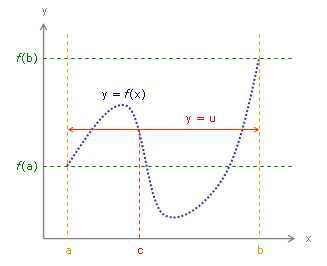
\includegraphics[scale=0.3]{images/025.png}
\end{wrapfigure} 

\bigskip\bigskip
cas n$^{\circ}$1 : Étirement, $x-x_{0}>0$,\\$\vec{F}$ dans le sens de $-\vec{i}$.

\bigskip\bigskip\bigskip\bigskip\bigskip\bigskip

cas n$^{\circ}$2 : Ressort au repos, $\vec{F}=\vec{0}$.\\\\

\bigskip\bigskip\bigskip\bigskip

cas n$^{\circ}$3 : Compression, $x-x_{0}<0$,\\$\vec{F}$ dans le sens de $\vec{i}$.\\\\

\subsection{Description mécanique du mouvement}
On considère le système \{ressort\} comme un système conservatif : $\frac{dE_{m}}{dt}=0$.\\

$E_{m}=E_{c}+E_{p}$ avec $\Delta E_{c}=\sum W_{\vec{F}_{ext}}$ et $\Delta E_{p}=-\sum W_{\vec{F}_{ext}}$.

\begin{center} \begin{tikzpicture}[scale=2]
\draw [domain=0:3*pi/5, samples=300] plot (\x,{sin(\x*20 r)/5}) ;
\draw (-0.5,-0.35) -- (-0.5,0.4) ;
\draw (-0.5,0) -- (0,0) ;
\draw (-0.7,-0.35) -- (3,-0.35) ;
\draw (2,-0.34) -- (2,0.26) -- (2.6,0.26) -- (2.6,-0.34) -- cycle ;
\draw (1.88,0) -- (2,0) ;
\draw[dashed] (1.02,-0.35) -- (1.02,0.49) ;
\node at (1.02,-0.5) {$x_{0}$} ;
\draw[>=latex, ->, thick] (2.3,-0.04) -- (2.3,-1) node[near end, below left] {$\vec{P}$};
\draw[>=latex, ->, thick] (2.4,-0.35) -- (2.4,0.65) node[near end, right] {$\vec{N}$};
\draw[>=latex, ->, thick] (2.31,-0.04) -- (1.6,-0.04) node[near end, above] {$\vec{F}$};
\end{tikzpicture} \end{center}

\bigskip\bigskip\bigskip

\subsubsection{Approche énergétique}
\textit{Calculons le travail des forces appliquées au système \{ressort\} pendant le mouvement}\\

Pour une position x quelconque, $x_{0}=0$ étant la position d'équilibre:\\

$W_{\vec{P}}=0$ car $\vec{P}$ est perpendiculaire au déplacement.

$W_{\vec{N}}=0$ car $\vec{N}$ est perpendiculaire au déplacement.

$\displaystyle W_{\vec{F}}=\int \vec{F}\cdot d\vec{x}=\int -kx\vec{i}\cdot dx\vec{i}=\int -kx \, dx=-\frac{1}{2}kx^{2}+C$.\\
Or pour $x_{0}=0$, $W_{\vec{F}}=0$ donc $C=0$ d'où $W_{\vec{F}}=-\frac{1}{2}kx^{2}$.\\\\

$\begin{array}{rcl} \text{Calcul de }W_{\vec{F}_{x_{i}\rightarrow x_{f}}}\text{ : }W_{\vec{F}_{x_{i}\rightarrow x_{f}}}&=&\displaystyle\int_{x_{i}}^{x_{f}} \vec{F}\cdot d\vec{x}\\\\
&=&\displaystyle\int_{x_{i}}^{x_{f}} -kx\vec{i}\cdot dx\vec{i}\\\\
&=&[-\frac{1}{2}kx^{2}]_{x_{i}}^{x_{f}}\\\\
&=&-\frac{1}{2}k(x_{f}^{2}-x_{i}^{2}) \end{array}$\\\\

La force de rappel est une force conservative : $\vec{F}_{x}=-\overrightarrow{\mathcal{G}\text{rad}}\,E_{p}=-\frac{dE_{p}}{dx}\vec{i}$ et $W_{\vec{F}}=-\Delta E_{p}$.\\

Choisissons $E_{p}(x_{0})=0$, dans ce cas $\Delta E_{p}=E_{p}(x)-E_{p}(x_{0})$.\\

Comme $W_{\vec{F}}=-\frac{1}{2}kx^{2}$ alors $\Delta E_{p}=E_{p}(x)+\frac{1}{2}kx^{2}\text{ et }E_{c}=\frac{1}{2}mv^{2}$.\\

$E_{m}=E_{p}+E_{c}=\frac{1}{2}kx^{2}+\frac{1}{2}mv^{2}$ or $\frac{dE_{m}}{dt}=0$\\

On dérive : $(\frac{1}{2}kx(t)^{2}+\frac{1}{2}mv(t)^{2})$ par rapport au temps :\\

$\begin{array}{rcl} &&\frac{dE_{m}}{dt}=\frac{1}{2}k\cdot 2\dot{x}(t)x(t)+\frac{1}{2}m\cdot 2\dot{v}(t)v(t)=0\\
&\Leftrightarrow &kx(t)+m\dot{v}(t)=0\\
&\Leftrightarrow &\ddot{x}(t)+\frac{k}{m}x(t)=0 \end{array}$\\

\begin{center} \begin{tikzpicture}[scale=1.5]
\draw [->,>=latex] (-3.5,-1) -- (3.4,-1) ;
\draw [->,>=latex] (0,-1.5) -- (0,2) ;
\node at (3.8,-1) {$x$(m)} ;
\node at (0.5,2) {E(J)} ;
\draw [color=green] (-3.15,1) -- (3.1415926535,1) ;
\draw [domain=-3.15:pi, samples=75, color=red] plot (\x,{cos(\x r)}) ;
\draw [domain=-3.15:pi, samples=75, color=blue] plot (\x,{-cos(\x r)}) ;
\node [color=green] at (3.5,1) {$E_{m}$} ;
\node [color=red] at (2.5,-0.4) {$E_{c}$} ;
\node [color=blue] at (2.5,0.4) {$E_{p}$} ;
\node at (0.25,-1.3) {$x_{0}$} ;
\node at (3.15,-1.072) {$\shortmid$} ;
\node at (3.15,-1.3) {$x_{max}$} ;
\node at (-3.15,-1.072) {$\shortmid$} ;
\node at (-3.15,-1.3) {$x_{min}$} ;
\draw[dashed] (-1,-1.1) -- (-1,1.5) ;
\node at (-1,-1.3) {$x_{2}$} ;
\draw[dashed] (1,-1.1) -- (1,1.5) ;
\node at (1,-1.3) {$x_{1}$} ;
\end{tikzpicture} \end{center}
\bigskip

En $x_{1}$, $\frac{dE_{p}(x_{1})}{dx}>0$ donc $\vec{F}$ est dans le sens des x décroissants.

En $x_{2}$, $\frac{dE_{p}(x_{2})}{dx}<0$ donc $\vec{F}$ est dans le sens des x croissants.\\\\
Un \textbf{équilibre stable} est défini lorsqu'un système un peu écarté de sa position d'équilibre y revient.\\

\subsubsection{Approche dynamique}
\textit{Utilisation du principe fondamental de la dynamique}\\

Le système est le \{ressort\} de masse m étudié dans le référentiel terrestre considéré galiléen.

\begin{center} \begin{tikzpicture}[scale=1.9]
\draw [domain=0:3*pi/5, samples=300] plot (\x,{sin(\x*20 r)/5}) ;
\draw (-0.5,-0.35) -- (-0.5,0.4) ;
\draw (-0.5,0) -- (0,0) ;
\draw[>=latex,->] (-0.7,-0.35) -- (3,-0.35) ;
\draw[thick, ->] (1.02,-0.35) -- (1.27,-0.35) node[above] {$\vec{i}$} ;
\draw (2,-0.34) -- (2,0.26) -- (2.6,0.26) -- (2.6,-0.34) -- cycle ;
\draw (1.88,0) -- (2,0) ;
\draw[>=latex,->] (1.02,-0.45) -- (1.02,0.49) ;
\draw[thick, ->] (1.02,-0.35) -- (1.02,-0.1) node[midway, left] {$\vec{j}$} ;
\node at (0.975,-0.5) {$x_{0}=0$} ;
\draw[->, thick] (2.3,-0.04) -- (2.3,-0.5) node[near end, below left] {$\vec{P}$};
\draw[->, thick] (2.4,-0.35) -- (2.4,0.65) node[near end, right] {$\vec{N}$};
\draw[->, thick] (2.308,-0.04) -- (1.76,-0.04) node[near end, above] {$\vec{F}$};
\draw[dashed] (2.32,0.8) -- (2.32,-0.4) ;
\node at (2.225,0.9) {$x(t=0)=X_{max}$} ;
\node at (1.15,0.5) {$O_{y}$} ;
\node at (3.05,-0.25) {$O_{x}$} ;
\end{tikzpicture} \end{center}

On applique le PFD : $\sum \vec{F}_{ext}=\vec{P}+\vec{N}+\vec{F}=\vec{F}=m\vec{a}$ car $\vec{P}+\vec{N}=\vec{0}$ puisqu'il n'y a pas de mouvement sur $O_{y}$.\\

$\vec{F}=m\vec{a} \Leftrightarrow -kx\,\vec{i}=ma\,\vec{i}$\\

$\begin{array}{rcl} \text{On projette selon } O_{x} \text{ : } &&-kx=ma \\
&\Leftrightarrow &-kx=m \ddot{x} \\
&\Leftrightarrow &\ddot{x}+\frac{k}{m}x=0 \end{array}$

\subsection{Résolution de l'équation différentielle}
Solution de la forme $x(t)=Acos(\omega t+\phi)$. $\phi$ est la phase (le décalage temporel),\\$\omega$ est la pulsation, A est l'amplitude du mouvement, la période T vaut $T=\frac{2\pi}{\omega}$.\\

On cherche quel est le lien entre A, $\omega$ et $\phi$, et k et m.\\

Si $x(t)=Acos(\omega t+\phi)$ est solution de $\ddot{x}+\frac{k}{m}x=0$ alors x(t) vérifie l'équation.\\

$\begin{array}{rcl} \ddot{x}=-A\omega^{2}\,cos(\omega t+\phi)\text{ donc on a }&&\ddot{x}+\frac{k}{m}x=0 \\
&\Leftrightarrow &A\,cos(\omega t+\phi)(-\omega^{2}+\frac{k}{m})=0 \\
&\Leftrightarrow &\frac{k}{m}-\omega^{2}=0 \end{array}$\\

Ainsi x est solution si $\omega=\sqrt{\frac{k}{m}}$.\\

Conditions initiales : à $t=0$, lorsqu'on lâche le ressort en position étirée, $x(t=0)=X_{max}$, $v(t=0)=0 \Leftrightarrow \dot{x}(t=0)=-A\omega\sin(\phi)=0$.\\

On \textit{choisit} $\phi=0$, on a alors $A=X_{max}$. Ainsi $x(t)=X_{max}\cos(\sqrt{\frac{k}{m}}t)$.\\

Remarque : En réécrivant la solution de l'équation différentielle en $x(t)=\lambda cos(\omega t)+\mu sin(\omega t)$ (en développant le cosinus), il devient plus simple de déterminer les valeurs des constantes.

\begin{center} \begin{tikzpicture}[scale=0.65]
\draw [domain=0:4*pi, samples=300, thick] plot (\x,{2*sin(\x r)}) ;
\draw[>=latex,->] (0,-2.5) -- (0,3) ;
\draw[>=latex,->] (-1,0) -- (13,0) ;
\node at (13.2,-0.3) {t(s)} ;
\node at (0.6,3) {x(m)} ;
\draw[<->,very thick] (pi/2,0) -- (pi/2,2) node[midway, right] {A} ;
\draw[<->,very thick] (pi,0) -- (3*pi,0) node[midway, below right] {T} ;
\node at (-0.6,2) {$x_{max}$} ;
\node at (-0.6,-2) {$x_{min}$} ;
\draw[dashed] (0,2) -- (4*pi,2) ;
\draw[dashed] (0,-2) -- (4*pi,-2) ;
\node at (-0.15,-0.2) {0} ;
\end{tikzpicture} \end{center}

\section{Oscillations verticales}
\textit{Dans le cas d'un oscillateur harmonique}
\begin{center}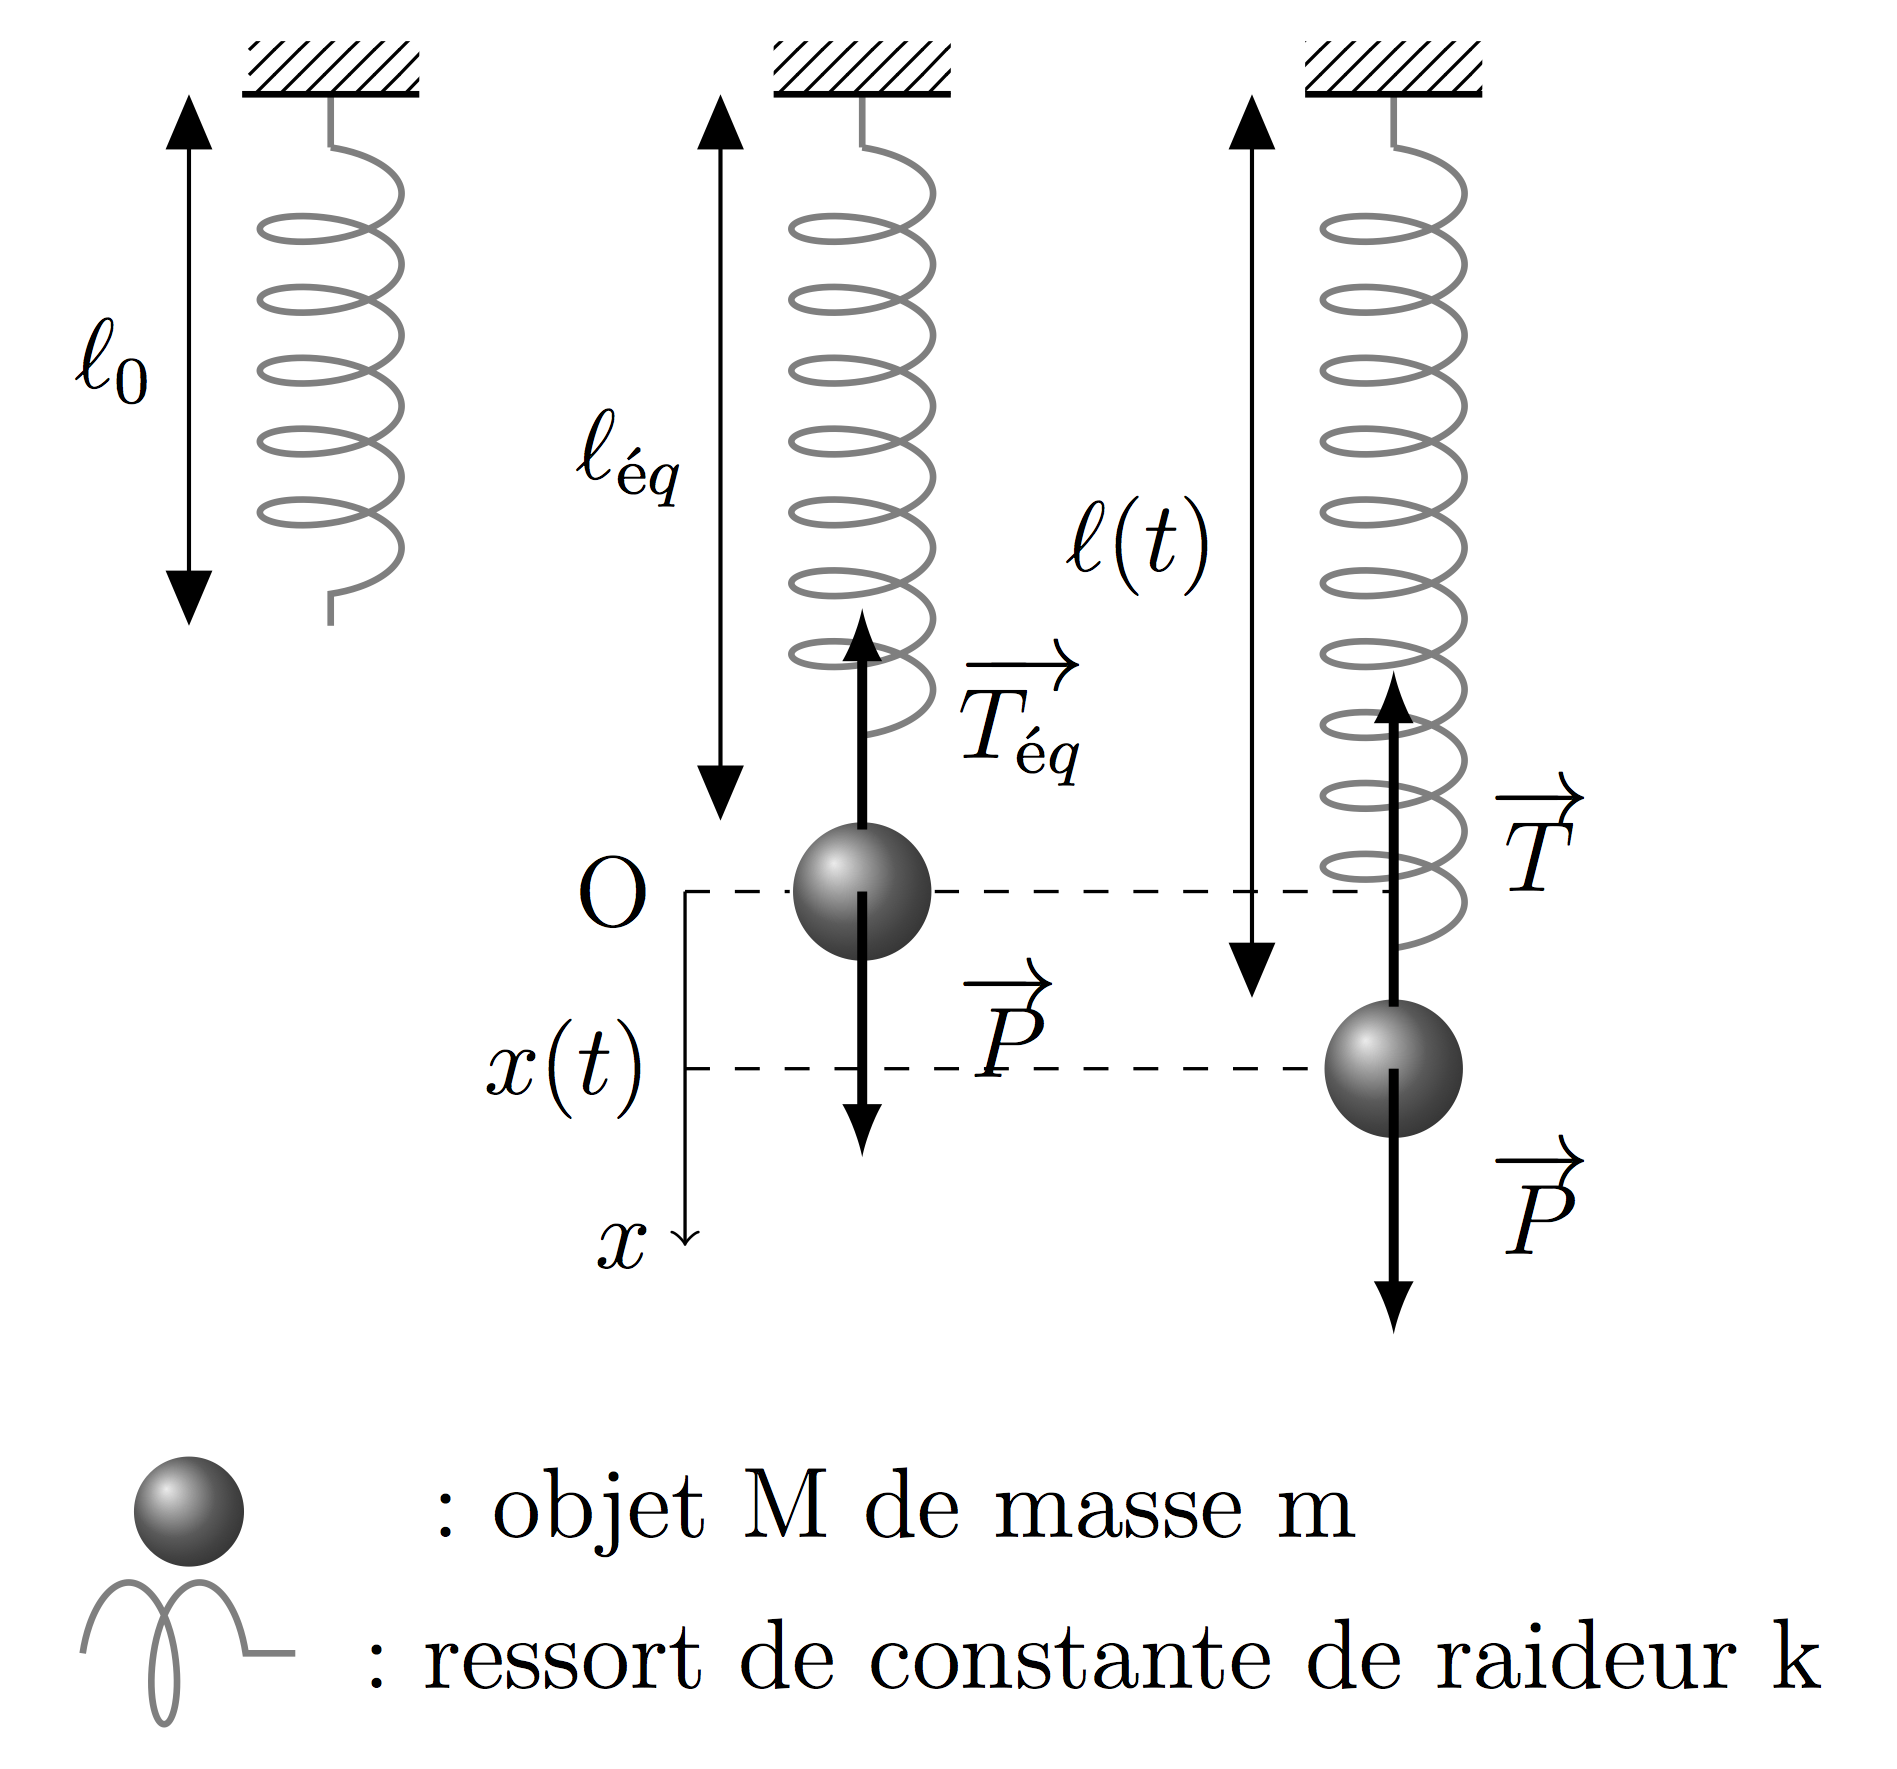
\includegraphics[scale=1.4]{images/026.png}\end{center}
\subsection{Description mécanique du mouvement}
On étudie le système {masse} suspendu à un ressort de masse négligeable dans le référentiel terrestre considéré comme galiléen auquel on associe un repère $H(O,O_{x})$.\\

\begin{itemize}
\item Cas du ressort à l'équilibre :\\

$\begin{array}{rcl}\text{D'après le principe fondamental de la dynamique on a } &&\sum \vec{F}=\vec{0}\\\\
&\Leftrightarrow& \vec{P}+\vec{F}=0\\\\
&\Leftrightarrow& mg-k(l_{éq}-l_{0})=0\\\\
&\Leftrightarrow& mg=k(l_{éq}-l_{0})\end{array}$ \bigskip

\item Cas du ressort hors équilibre :\\ \end{itemize}

On étire le ressort jusqu'à une longueur $l_{max}$ puis on lâche à t=0.\\

Pendant l'oscillation, d'après le principe fondamental de la dynamique on a $\vec{P}+\vec{F}=m\vec{a}$.\\
C'est-à-dire $mg-k(x-l_{0})=m\ddot{x}$.\\

Or à l'équilibre $mg=k(l_{éq}-l_{0})$, on a donc $kl_{éq}-kl_{0}-kx+kl_{0}=m\ddot{x}$\\
et donc $\ddot{x}+\frac{k}{m}x=\frac{kl_{éq}}{m}$.\\

\newpage

\subsection{Résolution de l'équation différentielle}
On cherche une solution du type $x(t)=Acos(\omega t+\phi)+l_{éq}$. On veut déterminer A, $\omega$ et $\phi$.\\\\

Pour trouver $\omega$, on remplace $x(t)$ et $\ddot{x}(t)$ dans l'équation différentielle :\\\\
$x(t)=Acos(\omega t +\phi )+l_{éq}$ donc $\dot{x}(t)=-A\omega sin(\omega t +\phi)$ et $\ddot{x}(t)=-A\omega^{2} cos(\omega t +\phi)$.\\\\
$\begin{array}{rcl} \text{Alors }\ddot{x}+\frac{k}{m}x=\frac{k}{m}l_{éq} &\Leftrightarrow &\frac{k}{m}Acos(\omega t +\phi )+\frac{k}{m}l_{éq}-A\omega^{2} cos(\omega t +\phi )=\frac{k}{m}l_{e}\\\\
&\Leftrightarrow& -\omega^{2}+\frac{k}{m}=0\\\\
&\Leftrightarrow& \omega =\sqrt{\frac{k}{m}}\end{array}$\\\\

Pour trouver $\phi$, on se place à $t=0$ où $v(t=0)=\dot{x}(t=0)=0$\\
or $\dot{x}(t)=A\omega sin(\omega t+\phi )$ donc $\dot{x}(t=0)=-A\omega sin(\phi)=0 \Leftrightarrow \phi= 0+k\pi$.\\\\

Pour trouver A, on se place à $t=0$, où $x(t=0)=l_{max}$,\\
or $x(t)=Acos(\omega t)+l_{éq}$ donc $x(t=0)=A cos(0)+l_{éq}=l_{max} \Leftrightarrow A=l_{max}-l_{éq}$.\\\\

Au final, $x(t)=(l_{max}-l_{éq})cos(\sqrt{\frac{k}{m}} t)+l_{éq}$.

\section{Oscillations amorties horizontales}
\subsection{Définition}
Un ressort oscille librement lorsqu'aucun frottement n'agit lors du mouvement.\\

A partir du moment où le mouvement d'oscillation se produit dans un milieu visqueux, les frottements ne peuvent plus être négligés et le mouvement d'oscillation s'amortit.\\

Étudier des oscillations amorties revient à définir des conditions pour lesquelles le régime d'amortissement est faible, fort ou critique.\\

\begin{center} \begin{tikzpicture}  
\draw (0,5) -- (0,0) -- (10,0) -- (10,5) ;
\draw[very thick] (1,0) -- (1,3) ;
\draw[thick] (1,1.5) -- (1.9,1.5) ;
\draw[thick] (5.03,1.5) -- (6,1.5) ;
\draw[thick] (6,0.05) -- (9,0.05) -- (9,3) -- (6,3) -- cycle ;
\draw [thick, domain=1.9:1.902+pi, samples=400] plot (\x,{sin((\x-1.9)*10 r)+1.5}) ;
\node at (5,4.75) {fluide visqueux} ;
\node at (4.85,4.4) {de coefficient de frottement $\alpha$} ;
\node at (7.5,2) {solide} ;
\node at (7.5,1.5) {de masse} ;
\node at (7.5,1) {m} ;
\node at (3.5,3.25) {ressort de constante} ;
\node at (3.5,2.9) {de raideur k} ;
\draw[->, very thick] (3,0) -- (3.5,0) ;
\node at (3.2,-0.2) {$\vec{i}$} ;
\end{tikzpicture} \end{center}

\newpage

\subsection{Description mécanique du mouvement}
On fait le bilan des forces appliquées sur le système {masse} :\\\\
Horizontalement : la force élastique (force de rappel du ressort) : $\vec{F}=-kx\vec{i}$ avec $x=l-l_{0}$\\
et la force de frottement : $\vec{f}=-\alpha v\vec{i}$.\\\\
Verticalement : le poids, la force normale du support et la poussée d'Archimède qui se compensent.\\

Si le mouvement est horizontal, le principe fondamental de la dynamique s'écrit $\vec{F}+\vec{f}=m\vec{a}$ c'est-à-dire $-kx\vec{i}-\alpha v \vec{i}=m\ddot{x} \vec{i}$ et donc $\ddot{x}+\frac{\alpha}{m}\dot{x}+\frac{k}{m}x=0$.

\subsection{Résolution de l'équation différentielle}
On obtient une équation du mouvement de m dans une situation d'amortissement.\\
On suppose que $x(t)=e^{ct}$ vérifie l'équation.\\

On réécrit l'équation en $\ddot{x}+\beta \dot{x}+\omega_{0}{}^{2}x=0$ avec $\omega_{0}$ la pulsation naturelle (qui serait celle du ressort s'il n'était pas amorti).\\

On remplace $x(t)=e^{ct}$ dans l'équation :\\
$c^{2}e^{ct}+\beta ce^{ct}+\omega_{0}{}^{2}e^{ct}=0$ donc $c^{2}+\beta c+\omega_{0}{}^{2}=0$.\\

Selon le signe du discriminant $\Delta=\beta^{2}-4\omega_{0}{}^{2}$, les solutions de l'équation différentielle sont différentes et donc la situation d'amortissement est différente :\\

$\Delta>0$ : amortissement critique.\\

$\Delta=0$ : amortissement fort.\\

$\Delta<0$ : amortissement faible.

\subsection{Cas de l'amortissement faible}
Dans le cas d'un amortissement faible, on a $\Delta<0$, on peut donc écrire $\Delta$ comme\\
$\Delta=\beta^{2}-4\omega_{0}{}^{2}=-(4\omega_{0}{}^{2}-\beta^{2})=i^{2}(4\omega_{0}{}^{2}-\beta^{2})$.\\

On a alors deux solutions complexes : $c_{1}=\frac{-\beta+i\sqrt{4\omega_{0}{}^{2}-\beta^{2}}}{2}$ et $c_{2}=\frac{-\beta-i\sqrt{4\omega_{0}{}^{2}-\beta^{2}}}{2}$,\\\\
et donc deux solutions de l'équation différentielle : $x_{1}(t)=e^{c_{1}t}$ et $x_{2}(t)=e^{c_{2}t}$.\\\\

On sait que la solution de l'équation différentielle est une combinaison linéaire des deux solutions ainsi obtenues donc on a $x(t)=A_{1}e^{c_{1}t}+A_{2}e^{c_{2}t}$.\\

On pose $\omega_{A}=\sqrt{4w_{0}{}^{2}-\beta^{2}}$ et on admet $A_{1}=\frac{A_{0}}{2}e^{i\phi}$ et $A_{2}=\frac{A_{0}}{2}e^{-i\phi}$.\\

$\begin{array}{rcl} \text{On a alors } && x(t)=\frac{A_{0}}{2}e^{i\phi}e^{\frac{-\beta+\omega_{A}}{2}t}+\frac{A_{0}}{2}e^{-i\phi}e^{\frac{-\beta-\omega_{A}}{2}t}\\\\
&\Leftrightarrow & x(t)=\frac{A_{0}}{2}e^{-\frac{\beta}{2}t}(e^{i(\phi +\frac{\omega_{A}}{2}t)}+e^{-i(\phi+\frac{\omega_{A}}{2}t)}) \\\\
&\Leftrightarrow & x(t)=A_{0}e^{-\frac{\beta}{2}t}\cos(\frac{\omega_{A}}{2}t+\phi)\text{ d'après les formules d'Euler.} \end{array}$\\\\\\\\

On veut maintenant déterminer les valeurs des constantes $\phi$ et $A_{0}$, on se sert des conditions initiales : $x(t=0)=x_{0}$ et $\dot{x}(t=0)=0$. \\\\\\

Pour trouver $\phi$, on commence par déterminer l'expression de $\dot{x}(t)$ : \\\\
$\dot{x}(t)=-\frac{\beta}{2}A_{0}e^{-\frac{\beta}{2}t}\cos(\frac{\omega_{A}}{2}t+\phi)-\frac{\omega}{2}A_{0}e^{-\frac{\beta}{2}t}\sin(\frac{\omega_{A}}{2}t+\phi)\\\\
\dot{x}(t)=-\frac{A_{0}}{2}e^{-\frac{\beta}{2}t}(\beta\cos(\frac{\omega_{A}}{2}t+\phi)+\omega\sin(\frac{\omega_{A}}{2}t+\phi))$\\\\

On utilise maintenant les conditions initiales :\\\\
$\begin{array}{rcl} \dot{x}(t=0)=0 &\Leftrightarrow &\beta *\cos(\phi)+\sin(\phi)\omega_{A}=0\\\\
&\Leftrightarrow &\tan(\phi)=-\frac{\beta}{\omega_{A}} \text{ et donc }\phi=-\arctan(\frac{\beta}{\omega_{A}}). \end{array}$\\\\

On utilise l'autre condition initiale pour déterminer la valeur de $A_{0}$ :\\\\
$\begin{array}{rcl} x(t=0)=x_{0} &\Leftrightarrow &A_{0}*\cos(\phi)=x_{0}\\\\
&\Leftrightarrow &A_{0}\cos(\arctan(\frac{\beta}{\omega_{A}}))=x_{0} \text{ or }\cos(\arctan(x))=\frac{1}{\sqrt{x^{2}+1}} \\\\
&\Leftrightarrow &A_{0}=x_{0}\sqrt{(\frac{\beta}{\omega_{A}})^{2}+1}\end{array}$\\\\\\

On a ainsi obtenu que dans le cas de l'amortissement faible d'une oscillation amortie, pour un système de masse m avec un ressort de constante de raideur k et un fluide de coefficient de frottement $\alpha$, avec $x_{0}=x(t=0)$ la position initiale du ressort, on a $x(t)=A_{0}e^{-\frac{\beta}{2}t}\cos(\frac{\omega_{A}}{2}t+\phi)$\\
avec $\beta=\frac{\alpha}{m}$, $\omega_{0}{}^{2}=\frac{k}{m}$, $\omega_{A}=\sqrt{(2\omega_{0})^{2}-\beta^{2}}$, $A_{0}=x_{0}\sqrt{(\frac{\beta}{\omega_{A}})^{2}+1}$ et $\phi=-\arctan(\frac{\beta}{\omega_{A}})$.\\\\\\

La pseudo-période de l'oscillation est $T=\frac{2\pi}{\omega_{A}}$.\\

\begin{center} \begin{tikzpicture}[scale=2.5]
\draw[->] (0,0) -- (5.05,0) ;
\node at (5,-0.15) {t(s)} ;
\draw[<->,>=latex,thick] (-0.05,0) -- (-0.05,1) node[midway, left] {$x_{0}$};
\draw [domain=0:5, samples=300] plot (\x,{exp(-\x)}) ;
\draw [thick, domain=0:5, samples=300] plot (\x,{exp(-\x)*cos(\x*10 r)}) ;
\draw [domain=0:5, samples=300] plot (\x,{-exp(-\x)}) ;
\draw[thick, <->, >=latex] (0.3,-0.74) -- (0.935,-0.74) node[midway, below] {T} ;
\draw[densely dashed] (0.935,-0.74) -- (0.935,-0.4) ;
\draw[->] (0,-1.2) -- (0,1.2) ;
\node at (0.25,1.15) {x(m)} ;
\end{tikzpicture} \end{center}

\newpage

\subsection{Cas de l'amortissement fort}
Dans le cas de l'amortissement fort, le discriminant est nul, l'équation du second degré a donc une seule racine $-\frac{\beta}{2}$ et la solution est de la forme $x(t)=(At+B)e^{-\frac{\beta}{2}t}$.\\

On utilise les conditions initiales pour déterminer les valeurs des constantes A et B ;\\
on sait que $x(t=0)=x_{0}$ et $v(t=0)=0$.\\

On a $x(t)=(At+B)e^{-\frac{\beta}{2}t}$ et donc $\dot{x}(t)=Ae^{-\frac{\beta}{2}t}-\frac{\beta}{2}(At+B)e^{-\frac{\beta}{2}t}$.\\

Ainsi on a $x(t=0)=B=x_{0}$ et ensuite $\dot{x}(t=0)=A-\frac{\beta}{2}B=0 \Leftrightarrow A=\frac{\beta}{2}x_{0}$.\\

On a ainsi obtenu que dans le cas de l’amortissement fort d’une oscillation amortie, pour un système de masse m avec un ressort de constante de raideur k et un fluide de coefficient de frottement $\alpha$, avec $x_{0}=x(t=0)$ la position initiale du ressort, on a $x(t)=(At+B)e^{-\frac{\beta}{2}t}$\\
avec $\beta=\frac{\alpha}{m}$, $A=\frac{\beta}{2}x_{0}$ et $B=x_{0}$.\\

Lorsque ce régime est atteint, l'oscillateur revient à sa position d'équilibre en un temps minimal.

\subsection{Cas de l'amortissement critique (ou apériodique)}
Dans le cas de l'amortissement critique, le discriminant est positif et donc il existe deux solutions réelles
de l'équation du second degré $c_{1}=\frac{-\beta +\sqrt{\beta^{2}-4\omega_{0}{}^{2}}}{2}$ et $c_{2}=\frac{-\beta -\sqrt{\beta^{2}-4\omega_{0}{}^{2}}}{2}$.\\

On en déduit ainsi deux solutions particulières de l'équation différentielle : $e^{c_{1}t}$ et $e^{c{2}t}$.\\\\
La solution est une combinaison linéaire des deux solutions obtenues :\\
$x(t)=e^{-\frac{\beta}{2}t}(Ae^{-t\sqrt{\frac{\beta^{2}}{4}-\omega_{0}{}^{2}}}+Be^{t\sqrt{\frac{\beta^{2}}{4}-\omega_{0}{}^{2}}})=e^{-\frac{\beta}{2}t}(Ae^{-\omega t}+Be^{\omega t})$ avec $\omega=\sqrt{\frac{\beta^{2}}{4}-\omega_{0}{}^{2}}$.\\

On applique alors les conditions initiales pour déterminer les valeurs des constantes A et B :\\
on sait que $x(t=0)=x_{0}$ et $v(t=0)=0$, de plus $x(t)=e^{-\frac{\beta}{2}t}(Ae^{-\omega t}+Be^{\omega t})$ et\\
$\dot{x}(t)=e^{-\frac{\beta}{2}t}[Be^{\omega t}(\omega-\frac{\beta}{2})-Ae^{-\omega t}(\omega+\frac{\beta}{2})]$.\\\\
$\left \{ \begin{array}{rcl}
x(t=0)&=&x_{0}\\
\dot{x}(t=0)&=&0\\
\end{array} \right. \Rightarrow \left \{ \begin{array}{rcl}
A+B&=&x_{0} \\
B(\omega-\frac{\beta}{2})&=&A(\omega+\frac{\beta}{2}) \\
\end{array} \right. \Rightarrow \left \{ \begin{array}{rcl}
A&=&x_{0}-B\\
2\omega B&=&x_{0}(\omega+\frac{\beta}{2}) \\
\end{array} \right. \Rightarrow \left \{ \begin{array}{rcl}
A&=&\frac{x_{0}}{2}(1-\frac{\beta}{2\omega}) \\
B&=&\frac{x_{0}}{2}(1+\frac{\beta}{2\omega}) \\
\end{array} \right.$

\bigskip

On a ainsi obtenu que dans le cas de l’amortissement critique d’une oscillation amortie, pour un système de masse m avec un ressort de constante de raideur k et un fluide de coefficient de frottement $\alpha$, avec $x_{0}=x(t=0)$ la position initiale du ressort, on a $x(t)=e^{-\frac{\beta}{2}t}(Ae^{-\omega t}+Be^{\omega t})$\\
avec $\beta=\frac{\alpha}{m}$, $\omega_{0}{}^{2}=\frac{k}{m}$, $\omega=\sqrt{\beta^{2}-4\omega_{0}{}^{2}}$, $A=\frac{x_{0}}{2}(1-\frac{\beta}{2\omega})$ et $B=\frac{x_{0}}{2}(1+\frac{\beta}{2\omega})$.

\begin{center}
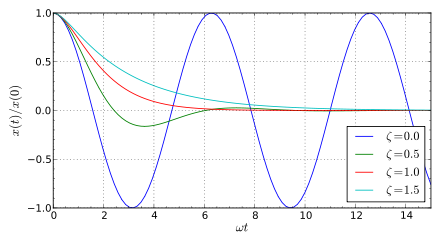
\includegraphics[scale=0.63]{images/027.png}
\end{center}
En bleu foncé une oscillation non amortie. En vert un amortissement faible.\\
En rouge un amortissement fort. En cyan un amortissement critique.

\section{Oscillations forcées horizontales}
\subsection{Sans frottements}
\subsubsection{Étude dynamique et définitions}
On parle d'oscillations forcées lorsque l'on applique à une masse accrochée à un ressort une force sinusoïdale telle que $||\vec{f}||=f_{0}\sin(\omega t)$.\\

\begin{center} \begin{tikzpicture}[scale=2.5]
\draw [domain=0:3*pi/5, samples=300] plot (\x,{sin(\x*20 r)/5}) ;
\draw (-0.5,-0.35) -- (-0.5,0.4) ;
\draw (-0.5,0) -- (0,0) ;
\draw[->] (-0.7,-0.35) -- (3,-0.35) ;
\draw (2,-0.34) -- (2,0.26) -- (2.6,0.26) -- (2.6,-0.34) -- cycle ;
\draw (1.88,0) -- (2,0) ;
\draw[>=latex, ->, thick] (2.3,-0.04) -- (2.3,-0.5) node[near end, below left] {$\vec{P}$};
\draw[>=latex, ->, thick] (2.35,-0.35) -- (2.35,0.25) node[near end, right] {$\vec{N}$};
\draw[>=latex, ->, thick] (2.306,-0.04) -- (1.8,-0.04) node[near end, above] {$\vec{F}$};
\node at (2.9,-0.45) {$x$} ;
\draw[->, >=latex, thick] (1.6,-0.15) -- (2,-0.15) node[midway,below] {$\vec{f}$} ;
\draw[->, thick] (1,-0.35) -- (1.2,-0.35) node[below, midway] {$\vec{i}$} ;
\end{tikzpicture} \end{center}

Il y a une force d'excitation de fréquence $\omega$ appliquée à une \{masse m\} accrochée à un ressort de constante de raideur k (et donc de fréquence propre $\omega_{0}=\sqrt{\frac{k}{m}}$).\\

Le but de l'étude est de décrire le mouvement de m selon les valeurs de $\omega_{0}$ et $\omega$.\\

Les seules forces qui agissent horizontalement sont la force de rappel du ressort $\vec{F}=-kx\vec{i}$ et la force excitatrice $\vec{f}=f_{0}\sin(\omega t)\vec{i}$ (on néglige les frottements).\\

On applique le principe fondamental de la dynamique : $\sum \vec{F}=m\vec{a}=-kx+f_{0}sin(\omega t)$\\
et donc $\ddot{x}+\frac{k}{m}\dot{x}=\frac{f_{0}}{m}sin(\omega t)$.

\subsubsection{Résolution de l'équation différentielle}
La solution est de la forme $x(t)=A\sin(\omega t+\phi)$. On cherche les valeurs de A et de $\phi$ :\\

On sait que $x(t)=A\sin(\omega t+\phi)$ et donc $\ddot{x}=-A\omega^{2}\sin(\omega t+\phi)$.\\

On injecte dans l'équation différentielle :\\
 
$\begin{array}{rcl} &&\ddot{x}+\frac{k}{m}\dot{x}=\frac{f_{0}}{m}sin(\omega t)\\\\
&\Leftrightarrow&-A\omega^{2}\sin(\omega t+\phi)+\frac{k}{m}A\sin(\omega t+\phi)=\frac{f_{0}}{m}\sin(\omega t)\\\\
&\Leftrightarrow& \sin(\omega t)(A\omega_{0}{}^{2}-A\omega^{2})\cos(\phi)+\cos(\omega t)\sin(\phi)(A\omega_{0}{}^{2}-A\omega^{2})=\frac{f_{0}}{m}\sin(\omega t)\end{array}$\\\\

On en déduit $\sin(\phi)=0$ (pour éliminer $\cos(\omega t)$) donc $\phi=0$ et donc\\
$(A\omega_{0}{}^{2}-A\omega^{2})\cos(\phi)=A\omega_{0}{}^{2}-A\omega^{2}=\frac{f_{0}}{m}$ d'où $A=\frac{f_{0}}{m(\omega_{0}{}^{2}-\omega^{2})}$.\\

\begin{center} \begin{tikzpicture}[scale=1.5]
\draw [thick, domain=-2:-0.1979, samples=400] plot (\x,{-1/(2*\x)}) ;
\draw [thick, domain=0.2:2, samples=300] plot (\x,{1/(2*\x)}) ;
\draw[dashed] (0,2.5) -- (0,0.1) ;
\node at (0,-0.15) {$\omega_{0}$} ;
\draw[->] (-2.1,0.05) -- (2.1,0.05) ;
\node at (2.15,-0.15) {$\omega$} ;
\draw[->] (-2,-0.1) -- (-2,2.75) node[near end, above left] {A} ;
\node at (-2.4,0.25) {$\frac{f_{0}}{m\omega_{0}{}^{2}}$} ;
\node at (0,2.75) {$\infty$} ;
\end{tikzpicture} \end{center}

\newpage

\subsection{Avec frottements}
Si l'on ajoute un frottement, l'équation différentielle devient $\ddot{x}+\frac{\alpha}{m}\dot{x}+\frac{k}{m}x=\frac{f_{0}}{m}\sin(\omega t)$.\\

Le phénomène de résonance se produit lorsque la force excitatrice que l'on applique à l'oscillateur agit à une fréquence $\omega$ égale à la fréquence propre de l'oscillateur, dans ce cas l'amplitude d'oscillation est maximale.\\

On utilise la notation complexe pour simplifier, la force excitatrice vaut alors $||\vec{f}||=f_{0}e^{i(\omega t-\frac{\pi}{2})}$ et la solution de l'équation est de la forme $x(t)=Ae^{i(\omega t +\phi)}$.\\
On a alors $\dot{x}=Ai\omega e^{i(\omega t +\phi)}$ et $\ddot{x}=-A\omega^{2} e^{i(\omega t +\phi)}$.\\

On injecte dans l'équation : $\ddot{x}+\frac{\alpha}{m}\dot{x}+\frac{k}{m}x=\frac{f_{0}}{m}e^{i(\omega t-\frac{\pi}{2})}$.\\\\
$\Leftrightarrow -A\omega^{2}e^{i\omega t}e^{i\phi}+i\frac{\alpha}{m}A\omega e^{i\omega t}e^{i\phi}+\omega_{0}{}^{2}Ae^{i\omega t}e^{i\phi}=\frac{f_{0}}{m}e^{i(\omega t-\frac{\pi}{2})}$\\\\
$\Leftrightarrow A(\omega_{0}{}^{2}+i\frac{\alpha}{m}-\omega^{2})e^{i\phi}=-i\frac{f_{0}}{m}$\\

$Ae^{i\phi}=\frac{f_{0}}{m}\frac{-i}{\omega_{0}{}^{2}-\omega^{2}+i\frac{\alpha}{m}\omega}=\frac{f_{0}}{m}\frac{i(\omega^{2}-\omega_{0}{}^{2})-\frac{\alpha}{m}\omega}{(\omega^{2}-\omega_{0}{}^{2})^{2}+(\frac{\alpha}{m}\omega)^{2}}$\\\\

Il faut maintenant isoler A et $\phi$, pour trouver A on se sert du module :\\\\
$\begin{array}{rcl} |Ae^{i\phi}|=|\frac{f_{0}}{m}\frac{i(\omega^{2}-\omega_{0}{}^{2})-\frac{\alpha}{m}\omega}{(\omega^{2}-\omega_{0}{}^{2})^{2}+(\frac{\alpha}{m}\omega)^{2}}|
&\Leftrightarrow& A=|\frac{f_{0}}{m}\frac{i(\omega^{2}-\omega_{0}{}^{2})-\frac{\alpha}{m}\omega}{(\omega^{2}-\omega_{0}{}^{2})^{2}+(\frac{\alpha}{m}\omega)^{2}}|=\frac{f_{0}}{m}\frac{\sqrt{(\omega^{2}-\omega_{0}{}^{2})^{2}+(\frac{\alpha}{m}\omega)^{2}}}{(\omega^{2}-\omega_{0}{}^{2})^{2}+(\frac{\alpha}{m}\omega)^{2}}\\\\
&\Leftrightarrow& A=\frac{f_{0}}{m\sqrt{(\omega^{2}-\omega_{0}{}^{2})^{2}+(\frac{\alpha}{m}\omega)^{2}}} \\\\ \end{array}$

Pour trouver $\phi$, on utilise l'argument et le fait que $\arg(a+ib)=\arctan(\frac{b}{a})$ :\\\\
$\arg(Ae^{i\phi})=\arg(\frac{f_{0}}{m}\frac{i(\omega^{2}-\omega_{0}{}^{2})-\frac{\alpha}{m}\omega}{(\omega^{2}-\omega_{0}{}^{2})^{2}+(\frac{\alpha}{m}\omega)^{2}}) \Leftrightarrow \phi=\arctan(\frac{\omega^{2}-\omega_{0}{}^{2}}{-\frac{\alpha}{m}\omega})$\\\\
et donc $\phi=\arctan(\frac{m(\omega_{0}{}^{2}-\omega^{2})}{\alpha\omega})$.\\\\\\

\begin{center} \begin{tikzpicture}[scale=2.5]
\draw [thick, domain=-1.5:-0.4, samples=400] plot (\x,{-1/(2*\x)}) ;
\draw [thick, domain=0.4:1.5, samples=300] plot (\x,{1/(2*\x)}) ;
\draw[dashed] (0,1.9) -- (0,0) ;
\node at (0,-0.15) {$\omega_{0}$} ;
\draw[->] (-2.1,0.05) -- (1.8,0.05) ;
\node at (1.8,-0.15) {$\omega$} ;
\draw[->] (-1.5,-0.1) -- (-1.5,2) node[near end, above left] {A} ;
\node at (-1.8,0.35) {$\frac{f_{0}}{m\omega_{0}{}^{2}}$} ;
\draw[thick] (-0.4,1.24) arc (172:8:0.405) ;
\end{tikzpicture} \end{center}





















\end{document}